%%%% Time-stamp: <2017-02-05 16:13:04 vk>
%% ========================================================================
%%%% Disclaimer
%% ========================================================================
%%
%% created by
%%
%%      Karl Voit
%%

%% ========================================================================
%%%% Basic settings
%% ========================================================================
%% (idea of using newcommands for basic documentclass settings from: Thomas Schlager)

\newcommand{\mypapersize}{A4}
%% e.g., "A4", "letter", "legal", "executive", ...
%% The size of the paper of the resulting PDF file.

%\newcommand{\mylaterality}{twoside}
\newcommand{\mylaterality}{oneside}
%% "oneside" or "twoside"
%% Either you are creating a document which is printed on both, left pages
%% and right pages (twoside) or you create a document which is printed
%% on right pages only (oneside).

\newcommand{\mydraft}{false}
%% "true" or "false"
%% Use draft mode? If true, included graphics are replaced by empty
%% rectangles (of same size) and overfull boxes (in margin space) are
%% marked with black box (-> easy to spot!)

\newcommand{\myparskip}{half}
%% e.g., "no", "full", "half", ...
%% How to separate paragraphs: indention ("no") or spacing ("half",
%% "full", ...).

\newcommand{\myBCOR}{0mm}
%% Inner binding correction. This value depends on the method which is
%% being used to bind your printed result. Some techniques do not
%% require a binding correction at all ("0mm"), other require for
%% example "5mm". Refer to KOMA script documentation for a detailed
%% explanation what a binding correction is and how to measure it.

\newcommand{\myfontsize}{11pt}
%% e.g., 10pt, 11pt, 12pt
%% The font size of the main text in pt (points).

\newcommand{\mylinespread}{1.0}
%% e.g., 1.0, 1.5, 2.0
%% Line spacing in %/100. For example 1.5 means 150% of the usual line
%% spacing. Please use with caution: 100% ("1.0") is fine because the
%% font was designed for it.

\newcommand{\mylanguage}{ngerman,american}
%% "english,ngerman", "ngerman,english", ...
%% NOTE: The *last* language is the active one!
%% See babel documentation for further details.

%% BibLaTeX-settings: (see biblatex reference for further description)
\newcommand{\mybiblatexstyle}{numeric}
%% e.g., "alphabetic", "authoryear", ...
%% The biblatex style which is being used for referencing. See
%% biblatex documentation for further details and more values.
%%
%% CAUTION: if you change the style, please check for (in)compatible
%%          "biblatex" package options in the file
%%          "template/preamble.tex"! For example: "alphabetic" does
%%          not have an option "dashed=..." and causes an error if it
%%          does not get removed from the list of options.

\newcommand{\mybiblatexdashed}{false}  %% "true" or "false"
%% If true: replace recurring reference authors with a dash.

\newcommand{\mybiblatexbackref}{true}  %% "true" or "false"
%% If true: create backward links from reference to citations.

% removed for vim-latex to find references
%\newcommand{\mybiblatexfile}{references-biblatex.bib}
%% Name of the biblatex file that holds the references.

%\newcommand{\mydispositioncolor}{30,103,182}
%% e.g., "30,103,182" (blue/turquois), "0,0,0" (black), ...
%% Color of the headings and so forth in RGB (red,green,blue) values.
%% NOTE: if you are using "0,0,0" for black, printers might still
%%       recognize pages as color pages. In case this is a problem
%%       (paying for color print-outs vs. paying for b/w-printouts)
%%       please edit file "template/preamble.tex" and change
%%       "\definecolor{DispositionColor}{RGB}{\mydispositioncolor}"
%%       to "\definecolor{DispositionColor}{gray}{0}" and thus
%%       overwriting the value of \mydispositioncolor above.

\newcommand{\mycolorlinks}{true}  %% "true" or "false"
%% Enables or disables colored links (hyperref package).

\newcommand{\mytitlepage}{template/title_Thesis_TU_Graz_-_kazemakase}
%% Your own or one of following pre-defined title pages:
%% "template/title_plain_maketitle": simple maketitle page
%% "template/title_Diplomarbeit_KF_Uni_Graz.tex": fancy (german) title page for KF Uni Graz
%% "template/title_Thesis_TU_Graz":
%%             titlepage for Graz University of Technology (correct
%%             (old?) Corporate Design) by Karl Voit (2012)
%% "template/title_Thesis_TU_Graz_-_kazemakase":
%%             titlepage for Graz University of Technology
%%             (correct new Corporate Design) by kazemakase (2013):
%%             see https://github.com/novoid/LaTeX-KOMA-template/issues/5
%% "template/title_VWA": titlepage for Vorwissenschaftliche Arbeit

\newcommand{\mytodonotesoptions}{}
%% e.g., "" (empty), "disable", ...
%% Options for the todonotes-package. If "disable", all todonotes will
%% be hidden (including listoftodos).

%% Load main settings for document preamble:
\input{template/preamble}%% DO NOT REMOVE THIS LINE!

% bibresource moved rere for vim-latex
\addbibresource{references-biblatex.bib} %% remove, if using BibTeX instead of biblatex

\setboolean{myaddcolophon}{false}  %% "true" or "false"
%% If set to "true": a colophon (with notes about this document
%% template, LaTeX, ...) is added after the title page.
%% Please do not set to "false" without a good reason. The colophon
%% helps your readers to get in touch with LaTeX and to find this template.

\setboolean{myaddlistoftodos}{true}  %% "true" or "false"
%% If set to "true": the current list of open todos is added after the
%% table of contents. If \mytodonotesoptions is set to "disable", no
%% list of todos is added, independent of this setting here.

\setboolean{english_affidavit}{true}  %% "true" or "false"
%% If set to "true": the language of the statutory declaration text is set to
%% English, otherwise it is in German.


%% ========================================================================
%%%% Document metadata
%% ========================================================================

%% general metadata:
\newcommand{\myauthor}{David Bidner}  %% also used for PDF metadata (hyperref)
\newcommand{\myauthorwithexistingtitles}{\myauthor{}, BSc}  %% including
                                %% university degree already held
                                %% (BSc, MSc, ...)
\newcommand{\mytitle}{Title TBD}  %% also used for PDF metadata (hyperref)
\newcommand{\mysubtitle}{Subtitle TBD}
\newcommand{\mysubject}{Subject TBD}  %% also used for PDF metadata (hyperref)
\newcommand{\mykeywords}{Keywords, TBD}  %% also used for PDF metadata (hyperref)

%% this information is used only for generating the title page:
\newcommand{\myworktitle}{Master's Thesis}  %% official type of work like ``Master theses''
\newcommand{\mygrade}{Diplom-Ingenieur} %% title you are getting with this work like ``Master of ...''
\newcommand{\mystudy}{Information and Computer Engineering} %% your study like ``Arts''
\newcommand{\mydegreeprogramme}{Master's degree programme: \mystudy} %% Master's or PhD degree programme
\newcommand{\myuniversity}{Graz University of Technology} %% your university/school
\newcommand{\myinstitute}{Institute of Applied Information Processing and Communications} %% affiliation
\newcommand{\myfaculty}{Faculty of Computer Science and Biomedical Engineering} % affiliation
%\newcommand{\myinstitutehead}{Univ.-Prof.\,Dipl-Ing.\,Dr.techn.~Some One} %% head of institute
\newcommand{\mysupervisor}{Dipl.-Ing. Dr.techn. Daniel Gruß} %% your supervisor
%\newcommand{\mycosupervisor}{Dr.~Some Body} %% your supervisor
\newcommand{\myevaluator}{Univ.-Prof. Dipl.-Ing. Dr.techn. Stefan Mangard} %% your evaluator
\newcommand{\myhomestreet}{} %% your home street (with house number)
\newcommand{\myhometown}{Graz} %% your home town
\newcommand{\myhomepostalnumber}{8010} %% your postal number of home town
\newcommand{\mysubmissionmonth}{TBD} %% month you are handing in
\newcommand{\mysubmissionyear}{2018} %% year you are handing in
\newcommand{\mysubmissiontown}{\myhometown} %% town of handing in (or \myhometown)

%% additional information for generic_documentation title page
\newcommand{\myid}{} %% Matrikelnummer
\newcommand{\mylecture}{LECTURE} %%


%% ========================================================================
%%%% MISC command definitions
%% ========================================================================
\input{template/mycommands}

%% ========================================================================
%%%% Typographic settings
%% ========================================================================
\input{template/typographic_settings}


%% ========================================================================
%%%% MISC usepackages
%% ========================================================================

%% ... it's OK to put here your own usepackage commands ...
\usepackage{subcaption}
\usepackage{amsmath,amssymb,amsfonts,xfrac}
\usepackage{tikz}
\usetikzlibrary{shapes.geometric, arrows, trees}
\usepackage{multirow}
\usepackage{booktabs}
\usepackage{circuitikz}
\usepackage{listings}
\usepackage{xcolor}

\tikzstyle{block} = [rectangle, minimum width=2cm, minimum height=0.8cm,
text centered, draw=black]
\tikzstyle{dot} = [circle, fill, inner sep=1.5pt]
\tikzstyle{function} = [rectangle, rounded corners, minimum width=2cm,
minimum height=0.8cm, text centered, draw=black, fill=blue!30]
\tikzstyle{arrow} = [thick,->,>=stealth]
\tikzset{XOR/.style={draw,circle,append after command={
        [shorten >=\pgflinewidth, shorten <=\pgflinewidth,]
        (\tikzlastnode.north) edge (\tikzlastnode.south)
        (\tikzlastnode.east) edge (\tikzlastnode.west)
        }
    }
}
\tikzstyle{level3block} = [rectangle, minimum width=9.5cm, minimum
height=0.8cm, text centered, draw=black]
\tikzstyle{mcblock} = [rectangle, minimum width=4cm, minimum
height=0.8cm, text centered, draw=black]
\tikzstyle{doublearrow} = [thick,<->,>=stealth]
\tikzstyle{segblock} = [rectangle, minimum width=1cm, minimum height=0.8cm,
text centered, draw=black]
\tikzstyle{memarray} = [rectangle, minimum width=3cm, minimum height=3cm,
                        text centered, draw=black]
\tikzstyle{memfunc} = [rectangle, minimum width=3cm, minimum height=1cm,
                       text centered, draw=black]
\tikzstyle{memcon} = [rectangle, minimum width=2cm, minimum height=2cm,
                        text centered, draw=black]
\tikzstyle{line} = [thick,-,>=stealth]
\tikzstyle{root} = [rectangle, rounded corners, minimum
width=2cm, minimum height=0.8cm, text centered, draw=black, font=\Large,
fill=red!30]
\tikzstyle{decision} = [diamond, rounded corners, minimum width=2cm, text
centered, draw=black, fill=blue!30]
\tikzstyle{finish} = [rectangle, rounded corners, minimum
width=2cm, minimum height=0.8cm, text centered, draw=black, font=\Large,
fill=green!30]

\tikzstyle{fsnode}=[draw=black,thick,anchor=west]
\tikzstyle{selected}=[draw=red,fill=red!30]
\tikzstyle{optional}=[dashed,fill=gray!50]

\definecolor{mGreen}{rgb}{0,0.6,0}
\definecolor{mGray}{rgb}{0.5,0.5,0.5}
\definecolor{mPurple}{rgb}{0.58,0,0.82}
\definecolor{backgroundColour}{rgb}{0.95,0.95,0.92}

\lstdefinestyle{CStyle}{
  backgroundcolor=\color{backgroundColour},
  commentstyle=\color{mGreen},
  keywordstyle=\color{magenta},
  numberstyle=\tiny\color{mGray},
  stringstyle=\color{mPurple},
  basicstyle=\footnotesize\ttfamily,
  breakatwhitespace=false,
  breaklines=true,
  captionpos=b,
  keepspaces=true,
  numbers=left,
  numberstyle=\tiny,
  numbersep=5pt,
  showspaces=false,
  showstringspaces=false,
  showtabs=false,
  tabsize=2,
  frame=lines,
  language=C
}
\definecolor{instruction}{RGB}{0,0,255} % blue
\definecolor{directive}{RGB}{128,0,128} % purple
\definecolor{register}{RGB}{128,0,0}    % dark red

\lstdefinestyle{nasm}{
  backgroundcolor=\color{backgroundColour},
  commentstyle=\color{mGreen},
  stringstyle=\color{mPurple},
  keywordstyle=\color{instruction},
  keywordstyle=[2]\color{directive},
  keywordstyle=[3]\color{register},
  basicstyle=\footnotesize\ttfamily,
  numbers=left,
  numberstyle=\tiny,
  numbersep=5pt,
  frame=lines,
  breaklines=true,
  prebreak=\raisebox{0ex}[0ex][0ex]{\ensuremath{\hookleftarrow}},
  showstringspaces=false,
  upquote=true,
  tabsize=2,
  captionpos=b,
  language=nasm
}

\definecolor{diffstart}{RGB}{0.5,0.5,0.5}
\definecolor{diffincl}{RGB}{128,0,0}
\definecolor{diffrem}{RGB}{128,0,128}

\lstdefinestyle{diff}{
  backgroundcolor=\color{backgroundColour},
  commentstyle=\color{mGreen},
  stringstyle=\color{mPurple},
  keywordstyle=\color{instruction},
  keywordstyle=[2]\color{directive},
  keywordstyle=[3]\color{register},
  basicstyle=\footnotesize\ttfamily,
  numbers=left,
  numberstyle=\tiny,
  numbersep=5pt,
  frame=lines,
  breaklines=true,
  prebreak=\raisebox{0ex}[0ex][0ex]{\ensuremath{\hookleftarrow}},
  showstringspaces=false,
  upquote=true,
  tabsize=2,
  captionpos=b,
  language=diff
}

\lstdefinelanguage{diff}{
  basicstyle=\footnotesize\ttfamily,
  morecomment=[f][\color{diffstart}]{@@},
  morecomment=[f][\color{diffincl}]{+\ },
  morecomment=[f][\color{diffrem}]{-\ },
}

\lstdefinelanguage{nasm}{
  sensitive=true,
  alsoletter={\%},
  % comments.
  %    ; line comment
  comment=[l]{;},
  % strings.
  %    "foo"
  %    'bar'
  string=[b]{"},
  morestring=[b]{'},
  % instructions.
  %    ref: http://www.nasm.us/doc/nasmdocb.html
  keywords=[1]{
AAA, AAD, AAM, AAS, ADC, ADCX, ADD, ADDPD, ADDPS, ADDSD, ADDSS, ADDSUBPD,
ADDSUBPS, ADOX, AESDEC, AESDECLAST, AESENC, AESENCLAST, AESIMC, AESKEYGENASSIST,
AND, ANDN, ANDNPD, ANDNPS, ANDPD, ANDPS, ARPL, BEXTR, BLCFILL, BLCI, BLCIC,
BLCMSK, BLCS, BLENDPD, BLENDPS, BLENDVPD, BLENDVPS, BLSFILL, BLSI, BLSIC,
BLSMSK, BLSR, BNDCL, BNDCN, BNDCU, BNDLDX, BNDMK, BNDMOV, BNDSTX, BOUND, BSF,
BSR, BSWAP, BT, BTC, BTR, BTS, BZHI, CALL, CBW, CDQ, CDQE, CLAC, CLC, CLD,
CLFLUSH, CLFLUSHOPT, CLGI, CLI, CLTS, CMC, CMOVA, CMOVAE, CMOVB, CMOVBE, CMOVC,
CMOVE, CMOVG, CMOVGE, CMOVL, CMOVLE, CMOVNA, CMOVNAE, CMOVNB, CMOVNBE, CMOVNC,
CMOVNE, CMOVNG, CMOVNGE, CMOVNL, CMOVNLE, CMOVNO, CMOVNP, CMOVNS, CMOVNZ, CMOVO,
CMOVP, CMOVPE, CMOVPO, CMOVS, CMOVZ, CMP, CMPEQPD, CMPEQPS, CMPEQSD, CMPEQSS,
CMPLEPD, CMPLEPS, CMPLESD, CMPLESS, CMPLTPD, CMPLTPS, CMPLTSD, CMPLTSS,
CMPNEQPD, CMPNEQPS, CMPNEQSD, CMPNEQSS, CMPNLEPD, CMPNLEPS, CMPNLESD, CMPNLESS,
CMPNLTPD, CMPNLTPS, CMPNLTSD, CMPNLTSS, CMPORDPD, CMPORDPS, CMPORDSD, CMPORDSS,
CMPPD, CMPPS, CMPSB, CMPSD, CMPSQ, CMPSS, CMPSW, CMPUNORDPD, CMPUNORDPS,
CMPUNORDSD, CMPUNORDSS, CMPXCHG, CMPXCHG16B, CMPXCHG486, CMPXCHG8B, COMISD,
COMISS, CPUID, CQO, CRC32, CVTDQ2PD, CVTDQ2PS, CVTPD2DQ, CVTPD2PI, CVTPD2PS,
CVTPI2PD, CVTPI2PS, CVTPS2DQ, CVTPS2PD, CVTPS2PI, CVTSD2SI, CVTSD2SS, CVTSI2SD,
CVTSI2SS, CVTSS2SD, CVTSS2SI, CVTTPD2DQ, CVTTPD2PI, CVTTPS2DQ, CVTTPS2PI,
CVTTSD2SI, CVTTSS2SI, CWD, CWDE, DAA, DAS, DEC, DIV, DIVPD, DIVPS, DIVSD, DIVSS,
DMINT, DPPD, DPPS, EMMS, ENTER, EXTRACTPS, EXTRQ, F2XM1, FABS, FADD, FADDP,
FBLD, FBSTP, FCHS, FCLEX, FCMOVB, FCMOVBE, FCMOVE, FCMOVNB, FCMOVNBE, FCMOVNE,
FCMOVNU, FCMOVU, FCOM, FCOMI, FCOMIP, FCOMP, FCOMPP, FCOS, FDECSTP, FDISI, FDIV,
FDIVP, FDIVR, FDIVRP, FEMMS, FENI, FFREE, FFREEP, FIADD, FICOM, FICOMP, FIDIV,
FIDIVR, FILD, FIMUL, FINCSTP, FINIT, FIST, FISTP, FISTTP, FISUB, FISUBR, FLD,
FLD1, FLDCW, FLDENV, FLDL2E, FLDL2T, FLDLG2, FLDLN2, FLDPI, FLDZ, FMUL, FMULP,
FNCLEX, FNDISI, FNENI, FNINIT, FNOP, FNSAVE, FNSTCW, FNSTENV, FNSTSW, FPATAN,
FPREM, FPREM1, FPTAN, FRNDINT, FRSTOR, FSAVE, FSCALE, FSETPM, FSIN, FSINCOS,
FSQRT, FST, FSTCW, FSTENV, FSTP, FSTSW, FSUB, FSUBP, FSUBR, FSUBRP, FTST, FUCOM,
FUCOMI, FUCOMIP, FUCOMP, FUCOMPP, FWAIT, FXAM, FXCH, FXRSTOR, FXRSTOR64, FXSAVE,
FXSAVE64, FXTRACT, FYL2X, FYL2XP1, GETSEC, HADDPD, HADDPS, HLT, HSUBPD, HSUBPS,
IBTS, ICEBP, IDIV, IMUL, IN, INC, INCBIN, INSB, INSD, INSERTPS, INSERTQ, INSW,
INT, INT01, INT03, INT1, INT3, INTO, INVD, INVEPT, INVLPG, INVLPGA, INVPCID,
INVVPID, IRET, IRETD, IRETQ, IRETW, JA, JAE, JB, JBE, JC, JCXZ, JE, JECXZ, JG,
JGE, JL, JLE, JMP, JMPE, JNA, JNAE, JNB, JNBE, JNC, JNE, JNG, JNGE, JNL, JNLE,
JNO, JNP, JNS, JNZ, JO, JP, JPE, JPO, JRCXZ, JS, JZ, KADDB, KADDD, KADDQ, KADDW,
KANDB, KANDD, KANDNB, KANDND, KANDNQ, KANDNW, KANDQ, KANDW, KMOVB, KMOVD, KMOVQ,
KMOVW, KNOTB, KNOTD, KNOTQ, KNOTW, KORB, KORD, KORQ, KORTESTB, KORTESTD,
KORTESTQ, KORTESTW, KORW, KSHIFTLB, KSHIFTLD, KSHIFTLQ, KSHIFTLW, KSHIFTRB,
KSHIFTRD, KSHIFTRQ, KSHIFTRW, KTESTB, KTESTD, KTESTQ, KTESTW, KUNPCKBW,
KUNPCKDQ, KUNPCKWD, KXNORB, KXNORD, KXNORQ, KXNORW, KXORB, KXORD, KXORQ, KXORW,
LAHF, LAR, LDDQU, LDMXCSR, LDS, LEA, LEAVE, LES, LFENCE, LFS, LGDT, LGS, LIDT,
LLDT, LLWPCB, LMSW, LOADALL, LOADALL286, LODSB, LODSD, LODSQ, LODSW, LOOP,
LOOPE, LOOPNE, LOOPNZ, LOOPZ, LSL, LSS, LTR, LWPINS, LWPVAL, LZCNT, MASKMOVDQU,
MASKMOVQ, MAXPD, MAXPS, MAXSD, MAXSS, MFENCE, MINPD, MINPS, MINSD, MINSS,
MONITOR, MONTMUL, MOV, MOVAPD, MOVAPS, MOVBE, MOVD, MOVDDUP, MOVDQ2Q, MOVDQA,
MOVDQU, MOVHLPS, MOVHPD, MOVHPS, MOVLHPS, MOVLPD, MOVLPS, MOVMSKPD, MOVMSKPS,
MOVNTDQ, MOVNTDQA, MOVNTI, MOVNTPD, MOVNTPS, MOVNTQ, MOVNTSD, MOVNTSS, MOVQ,
MOVQ2DQ, MOVSB, MOVSD, MOVSHDUP, MOVSLDUP, MOVSQ, MOVSS, MOVSW, MOVSX, MOVSXD,
MOVUPD, MOVUPS, MOVZX, MPSADBW, MUL, MULPD, MULPS, MULSD, MULSS, MULX, MWAIT,
NEG, NOP, NOT, OR, ORPD, ORPS, OUT, OUTSB, OUTSD, OUTSW, PABSB, PABSD, PABSW,
PACKSSDW, PACKSSWB, PACKUSDW, PACKUSWB, PADDB, PADDD, PADDQ, PADDSB, PADDSIW,
PADDSW, PADDUSB, PADDUSW, PADDW, PALIGNR, PAND, PANDN, PAUSE, PAVEB, PAVGB,
PAVGUSB, PAVGW, PBLENDVB, PBLENDW, PCLMULHQHQDQ, PCLMULHQLQDQ, PCLMULLQHQDQ,
PCLMULLQLQDQ, PCLMULQDQ, PCMPEQB, PCMPEQD, PCMPEQQ, PCMPEQW, PCMPESTRI,
PCMPESTRM, PCMPGTB, PCMPGTD, PCMPGTQ, PCMPGTW, PCMPISTRI, PCMPISTRM, PDEP,
PDISTIB, PEXT, PEXTRB, PEXTRD, PEXTRQ, PEXTRW, PF2ID, PF2IW, PFACC, PFADD,
PFCMPEQ, PFCMPGE, PFCMPGT, PFMAX, PFMIN, PFMUL, PFNACC, PFPNACC, PFRCP,
PFRCPIT1, PFRCPIT2, PFRCPV, PFRSQIT1, PFRSQRT, PFRSQRTV, PFSUB, PFSUBR, PHADDD,
PHADDSW, PHADDW, PHMINPOSUW, PHSUBD, PHSUBSW, PHSUBW, PI2FD, PI2FW, PINSRB,
PINSRD, PINSRQ, PINSRW, PMACHRIW, PMADDUBSW, PMADDWD, PMAGW, PMAXSB, PMAXSD,
PMAXSW, PMAXUB, PMAXUD, PMAXUW, PMINSB, PMINSD, PMINSW, PMINUB, PMINUD, PMINUW,
PMOVMSKB, PMOVSXBD, PMOVSXBQ, PMOVSXBW, PMOVSXDQ, PMOVSXWD, PMOVSXWQ, PMOVZXBD,
PMOVZXBQ, PMOVZXBW, PMOVZXDQ, PMOVZXWD, PMOVZXWQ, PMULDQ, PMULHRIW, PMULHRSW,
PMULHRWA, PMULHRWC, PMULHUW, PMULHW, PMULLD, PMULLW, PMULUDQ, PMVGEZB, PMVLZB,
PMVNZB, PMVZB, POP, POPA, POPAD, POPAW, POPCNT, POPF, POPFD, POPFQ, POPFW, POR,
PREFETCH, PREFETCHNTA, PREFETCHT0, PREFETCHT1, PREFETCHT2, PREFETCHW,
PREFETCHWT1, PSADBW, PSHUFB, PSHUFD, PSHUFHW, PSHUFLW, PSHUFW, PSIGNB, PSIGND,
PSIGNW, PSLLD, PSLLDQ, PSLLQ, PSLLW, PSRAD, PSRAW, PSRLD, PSRLDQ, PSRLQ, PSRLW,
PSUBB, PSUBD, PSUBQ, PSUBSB, PSUBSIW, PSUBSW, PSUBUSB, PSUBUSW, PSUBW, PSWAPD,
PTEST, PUNPCKHBW, PUNPCKHDQ, PUNPCKHQDQ, PUNPCKHWD, PUNPCKLBW, PUNPCKLDQ,
PUNPCKLQDQ, PUNPCKLWD, PUSH, PUSHA, PUSHAD, PUSHAW, PUSHF, PUSHFD, PUSHFQ,
PUSHFW, PXOR, RCL, RCPPS, RCPSS, RCR, RDFSBASE, RDGSBASE, RDM, RDMSR, RDPMC,
RDRAND, RDSEED, RDSHR, RDTSC, RDTSCP, RET, RETF, RETN, ROL, ROR, RORX, ROUNDPD,
ROUNDPS, ROUNDSD, ROUNDSS, RSDC, RSLDT, RSM, RSQRTPS, RSQRTSS, RSTS, SAHF, SAL,
SALC, SAR, SARX, SBB, SCASB, SCASD, SCASQ, SCASW, SETA, SETAE, SETB, SETBE,
SETC, SETE, SETG, SETGE, SETL, SETLE, SETNA, SETNAE, SETNB, SETNBE, SETNC,
SETNE, SETNG, SETNGE, SETNL, SETNLE, SETNO, SETNP, SETNS, SETNZ, SETO, SETP,
SETPE, SETPO, SETS, SETZ, SFENCE, SGDT, SHA1MSG1, SHA1MSG2, SHA1NEXTE,
SHA1RNDS4, SHA256MSG1, SHA256MSG2, SHA256RNDS2, SHL, SHLD, SHLX, SHR, SHRD,
SHRX, SHUFPD, SHUFPS, SIDT, SKINIT, SLDT, SLWPCB, SMI, SMINT, SMINTOLD, SMSW,
SQRTPD, SQRTPS, SQRTSD, SQRTSS, STAC, STC, STD, STGI, STI, STMXCSR, STOSB,
STOSD, STOSQ, STOSW, STR, SUB, SUBPD, SUBPS, SUBSD, SUBSS, SVDC, SVLDT, SVTS,
SWAPGS, SYSCALL, SYSENTER, SYSEXIT, SYSRET, T1MSKC, TEST, TZCNT, TZMSK, UCOMISD,
UCOMISS, UD0, UD1, UD2, UD2A, UD2B, UMOV, UNPCKHPD, UNPCKHPS, UNPCKLPD,
UNPCKLPS, VADDPD, VADDPS, VADDSD, VADDSS, VADDSUBPD, VADDSUBPS, VAESDEC,
VAESDECLAST, VAESENC, VAESENCLAST, VAESIMC, VAESKEYGENASSIST, VALIGND, VALIGNQ,
VANDNPD, VANDNPS, VANDPD, VANDPS, VBLENDMPD, VBLENDMPS, VBLENDPD, VBLENDPS,
VBLENDVPD, VBLENDVPS, VBROADCASTF128, VBROADCASTF32X2, VBROADCASTF32X4,
VBROADCASTF32X8, VBROADCASTF64X2, VBROADCASTF64X4, VBROADCASTI128,
VBROADCASTI32X2, VBROADCASTI32X4, VBROADCASTI32X8, VBROADCASTI64X2,
VBROADCASTI64X4, VBROADCASTSD, VBROADCASTSS, VCMPEQPD, VCMPEQPS, VCMPEQSD,
VCMPEQSS, VCMPFALSEPD, VCMPFALSEPS, VCMPFALSESD, VCMPFALSESS, VCMPGEPD,
VCMPGEPS, VCMPGESD, VCMPGESS, VCMPGTPD, VCMPGTPS, VCMPGTSD, VCMPGTSS, VCMPLEPD,
VCMPLEPS, VCMPLESD, VCMPLESS, VCMPLTPD, VCMPLTPS, VCMPLTSD, VCMPLTSS, VCMPNEQPD,
VCMPNEQPS, VCMPNEQSD, VCMPNEQSS, VCMPNGEPD, VCMPNGEPS, VCMPNGESD, VCMPNGESS,
VCMPNGTPD, VCMPNGTPS, VCMPNGTSD, VCMPNGTSS, VCMPNLEPD, VCMPNLEPS, VCMPNLESD,
VCMPNLESS, VCMPNLTPD, VCMPNLTPS, VCMPNLTSD, VCMPNLTSS, VCMPORDPD, VCMPORDPS,
VCMPORDSD, VCMPORDSS, VCMPPD, VCMPPS, VCMPSD, VCMPSS, VCMPTRUEPD, VCMPTRUEPS,
VCMPTRUESD, VCMPTRUESS, VCMPUNORDPD, VCMPUNORDPS, VCMPUNORDSD, VCMPUNORDSS,
VCOMISD, VCOMISS, VCOMPRESSPD, VCOMPRESSPS, VCVTDQ2PD, VCVTDQ2PS, VCVTPD2DQ,
VCVTPD2PS, VCVTPD2QQ, VCVTPD2UDQ, VCVTPD2UQQ, VCVTPH2PS, VCVTPS2DQ, VCVTPS2PD,
VCVTPS2PH, VCVTPS2QQ, VCVTPS2UDQ, VCVTPS2UQQ, VCVTQQ2PD, VCVTQQ2PS, VCVTSD2SI,
VCVTSD2SS, VCVTSD2USI, VCVTSI2SD, VCVTSI2SS, VCVTSS2SD, VCVTSS2SI, VCVTSS2USI,
VCVTTPD2DQ, VCVTTPD2QQ, VCVTTPD2UDQ, VCVTTPD2UQQ, VCVTTPS2DQ, VCVTTPS2QQ,
VCVTTPS2UDQ, VCVTTPS2UQQ, VCVTTSD2SI, VCVTTSD2USI, VCVTTSS2SI, VCVTTSS2USI,
VCVTUDQ2PD, VCVTUDQ2PS, VCVTUQQ2PD, VCVTUQQ2PS, VCVTUSI2SD, VCVTUSI2SS,
VDBPSADBW, VDIVPD, VDIVPS, VDIVSD, VDIVSS, VDPPD, VDPPS, VERR, VERW, VEXP2PD,
VEXP2PS, VEXPANDPD, VEXPANDPS, VEXTRACTF128, VEXTRACTF32X4, VEXTRACTF32X8,
VEXTRACTF64X2, VEXTRACTF64X4, VEXTRACTI128, VEXTRACTI32X4, VEXTRACTI32X8,
VEXTRACTI64X2, VEXTRACTI64X4, VEXTRACTPS, VFIXUPIMMPD, VFIXUPIMMPS, VFIXUPIMMSD,
VFIXUPIMMSS, VFMADD123PD, VFMADD123PS, VFMADD123SD, VFMADD123SS, VFMADD132PD,
VFMADD132PS, VFMADD132SD, VFMADD132SS, VFMADD213PD, VFMADD213PS, VFMADD213SD,
VFMADD213SS, VFMADD231PD, VFMADD231PS, VFMADD231SD, VFMADD231SS, VFMADD312PD,
VFMADD312PS, VFMADD312SD, VFMADD312SS, VFMADD321PD, VFMADD321PS, VFMADD321SD,
VFMADD321SS, VFMADDPD, VFMADDPS, VFMADDSD, VFMADDSS, VFMADDSUB123PD,
VFMADDSUB123PS, VFMADDSUB132PD, VFMADDSUB132PS, VFMADDSUB213PD, VFMADDSUB213PS,
VFMADDSUB231PD, VFMADDSUB231PS, VFMADDSUB312PD, VFMADDSUB312PS, VFMADDSUB321PD,
VFMADDSUB321PS, VFMADDSUBPD, VFMADDSUBPS, VFMSUB123PD, VFMSUB123PS, VFMSUB123SD,
VFMSUB123SS, VFMSUB132PD, VFMSUB132PS, VFMSUB132SD, VFMSUB132SS, VFMSUB213PD,
VFMSUB213PS, VFMSUB213SD, VFMSUB213SS, VFMSUB231PD, VFMSUB231PS, VFMSUB231SD,
VFMSUB231SS, VFMSUB312PD, VFMSUB312PS, VFMSUB312SD, VFMSUB312SS, VFMSUB321PD,
VFMSUB321PS, VFMSUB321SD, VFMSUB321SS, VFMSUBADD123PD, VFMSUBADD123PS,
VFMSUBADD132PD, VFMSUBADD132PS, VFMSUBADD213PD, VFMSUBADD213PS, VFMSUBADD231PD,
VFMSUBADD231PS, VFMSUBADD312PD, VFMSUBADD312PS, VFMSUBADD321PD, VFMSUBADD321PS,
VFMSUBADDPD, VFMSUBADDPS, VFMSUBPD, VFMSUBPS, VFMSUBSD, VFMSUBSS, VFNMADD123PD,
VFNMADD123PS, VFNMADD123SD, VFNMADD123SS, VFNMADD132PD, VFNMADD132PS,
VFNMADD132SD, VFNMADD132SS, VFNMADD213PD, VFNMADD213PS, VFNMADD213SD,
VFNMADD213SS, VFNMADD231PD, VFNMADD231PS, VFNMADD231SD, VFNMADD231SS,
VFNMADD312PD, VFNMADD312PS, VFNMADD312SD, VFNMADD312SS, VFNMADD321PD,
VFNMADD321PS, VFNMADD321SD, VFNMADD321SS, VFNMADDPD, VFNMADDPS, VFNMADDSD,
VFNMADDSS, VFNMSUB123PD, VFNMSUB123PS, VFNMSUB123SD, VFNMSUB123SS, VFNMSUB132PD,
VFNMSUB132PS, VFNMSUB132SD, VFNMSUB132SS, VFNMSUB213PD, VFNMSUB213PS,
VFNMSUB213SD, VFNMSUB213SS, VFNMSUB231PD, VFNMSUB231PS, VFNMSUB231SD,
VFNMSUB231SS, VFNMSUB312PD, VFNMSUB312PS, VFNMSUB312SD, VFNMSUB312SS,
VFNMSUB321PD, VFNMSUB321PS, VFNMSUB321SD, VFNMSUB321SS, VFNMSUBPD, VFNMSUBPS,
VFNMSUBSD, VFNMSUBSS, VFPCLASSPD, VFPCLASSPS, VFPCLASSSD, VFPCLASSSS, VFRCZPD,
VFRCZPS, VFRCZSD, VFRCZSS, VGATHERDPD, VGATHERDPS, VGATHERPF0DPD, VGATHERPF0DPS,
VGATHERPF0QPD, VGATHERPF0QPS, VGATHERPF1DPD, VGATHERPF1DPS, VGATHERPF1QPD,
VGATHERPF1QPS, VGATHERQPD, VGATHERQPS, VGETEXPPD, VGETEXPPS, VGETEXPSD,
VGETEXPSS, VGETMANTPD, VGETMANTPS, VGETMANTSD, VGETMANTSS, VHADDPD, VHADDPS,
VHSUBPD, VHSUBPS, VINSERTF128, VINSERTF32X4, VINSERTF32X8, VINSERTF64X2,
VINSERTF64X4, VINSERTI128, VINSERTI32X4, VINSERTI32X8, VINSERTI64X2,
VINSERTI64X4, VINSERTPS, VLDDQU, VLDMXCSR, VLDQQU, VMASKMOVDQU, VMASKMOVPD,
VMASKMOVPS, VMAXPD, VMAXPS, VMAXSD, VMAXSS, VMCALL, VMCLEAR, VMFUNC, VMINPD,
VMINPS, VMINSD, VMINSS, VMLAUNCH, VMLOAD, VMMCALL, VMOVAPD, VMOVAPS, VMOVD,
VMOVDDUP, VMOVDQA, VMOVDQA32, VMOVDQA64, VMOVDQU, VMOVDQU16, VMOVDQU32,
VMOVDQU64, VMOVDQU8, VMOVHLPS, VMOVHPD, VMOVHPS, VMOVLHPS, VMOVLPD, VMOVLPS,
VMOVMSKPD, VMOVMSKPS, VMOVNTDQ, VMOVNTDQA, VMOVNTPD, VMOVNTPS, VMOVNTQQ, VMOVQ,
VMOVQQA, VMOVQQU, VMOVSD, VMOVSHDUP, VMOVSLDUP, VMOVSS, VMOVUPD, VMOVUPS,
VMPSADBW, VMPTRLD, VMPTRST, VMREAD, VMRESUME, VMRUN, VMSAVE, VMULPD, VMULPS,
VMULSD, VMULSS, VMWRITE, VMXOFF, VMXON, VORPD, VORPS, VPABSB, VPABSD, VPABSQ,
VPABSW, VPACKSSDW, VPACKSSWB, VPACKUSDW, VPACKUSWB, VPADDB, VPADDD, VPADDQ,
VPADDSB, VPADDSW, VPADDUSB, VPADDUSW, VPADDW, VPALIGNR, VPAND, VPANDD, VPANDN,
VPANDND, VPANDNQ, VPANDQ, VPAVGB, VPAVGW, VPBLENDD, VPBLENDMB, VPBLENDMD,
VPBLENDMQ, VPBLENDMW, VPBLENDVB, VPBLENDW, VPBROADCASTB, VPBROADCASTD,
VPBROADCASTMB2Q, VPBROADCASTMW2D, VPBROADCASTQ, VPBROADCASTW, VPCLMULHQHQDQ,
VPCLMULHQLQDQ, VPCLMULLQHQDQ, VPCLMULLQLQDQ, VPCLMULQDQ, VPCMOV, VPCMPB, VPCMPD,
VPCMPEQB, VPCMPEQD, VPCMPEQQ, VPCMPEQW, VPCMPESTRI, VPCMPESTRM, VPCMPGTB,
VPCMPGTD, VPCMPGTQ, VPCMPGTW, VPCMPISTRI, VPCMPISTRM, VPCMPQ, VPCMPUB, VPCMPUD,
VPCMPUQ, VPCMPUW, VPCMPW, VPCOMB, VPCOMD, VPCOMPRESSD, VPCOMPRESSQ, VPCOMQ,
VPCOMUB, VPCOMUD, VPCOMUQ, VPCOMUW, VPCOMW, VPCONFLICTD, VPCONFLICTQ,
VPERM2F128, VPERM2I128, VPERMB, VPERMD, VPERMI2B, VPERMI2D, VPERMI2PD,
VPERMI2PS, VPERMI2Q, VPERMI2W, VPERMILPD, VPERMILPS, VPERMPD, VPERMPS, VPERMQ,
VPERMT2B, VPERMT2D, VPERMT2PD, VPERMT2PS, VPERMT2Q, VPERMT2W, VPERMW, VPEXPANDD,
VPEXPANDQ, VPEXTRB, VPEXTRD, VPEXTRQ, VPEXTRW, VPGATHERDD, VPGATHERDQ,
VPGATHERQD, VPGATHERQQ, VPHADDBD, VPHADDBQ, VPHADDBW, VPHADDD, VPHADDDQ,
VPHADDSW, VPHADDUBD, VPHADDUBQ, VPHADDUBW, VPHADDUDQ, VPHADDUWD, VPHADDUWQ,
VPHADDW, VPHADDWD, VPHADDWQ, VPHMINPOSUW, VPHSUBBW, VPHSUBD, VPHSUBDQ, VPHSUBSW,
VPHSUBW, VPHSUBWD, VPINSRB, VPINSRD, VPINSRQ, VPINSRW, VPLZCNTD, VPLZCNTQ,
VPMACSDD, VPMACSDQH, VPMACSDQL, VPMACSSDD, VPMACSSDQH, VPMACSSDQL, VPMACSSWD,
VPMACSSWW, VPMACSWD, VPMACSWW, VPMADCSSWD, VPMADCSWD, VPMADD52HUQ, VPMADD52LUQ,
VPMADDUBSW, VPMADDWD, VPMASKMOVD, VPMASKMOVQ, VPMAXSB, VPMAXSD, VPMAXSQ,
VPMAXSW, VPMAXUB, VPMAXUD, VPMAXUQ, VPMAXUW, VPMINSB, VPMINSD, VPMINSQ, VPMINSW,
VPMINUB, VPMINUD, VPMINUQ, VPMINUW, VPMOVB2M, VPMOVD2M, VPMOVDB, VPMOVDW,
VPMOVM2B, VPMOVM2D, VPMOVM2Q, VPMOVM2W, VPMOVMSKB, VPMOVQ2M, VPMOVQB, VPMOVQD,
VPMOVQW, VPMOVSDB, VPMOVSDW, VPMOVSQB, VPMOVSQD, VPMOVSQW, VPMOVSWB, VPMOVSXBD,
VPMOVSXBQ, VPMOVSXBW, VPMOVSXDQ, VPMOVSXWD, VPMOVSXWQ, VPMOVUSDB, VPMOVUSDW,
VPMOVUSQB, VPMOVUSQD, VPMOVUSQW, VPMOVUSWB, VPMOVW2M, VPMOVWB, VPMOVZXBD,
VPMOVZXBQ, VPMOVZXBW, VPMOVZXDQ, VPMOVZXWD, VPMOVZXWQ, VPMULDQ, VPMULHRSW,
VPMULHUW, VPMULHW, VPMULLD, VPMULLQ, VPMULLW, VPMULTISHIFTQB, VPMULUDQ, VPOR,
VPORD, VPORQ, VPPERM, VPROLD, VPROLQ, VPROLVD, VPROLVQ, VPRORD, VPRORQ, VPRORVD,
VPRORVQ, VPROTB, VPROTD, VPROTQ, VPROTW, VPSADBW, VPSCATTERDD, VPSCATTERDQ,
VPSCATTERQD, VPSCATTERQQ, VPSHAB, VPSHAD, VPSHAQ, VPSHAW, VPSHLB, VPSHLD,
VPSHLQ, VPSHLW, VPSHUFB, VPSHUFD, VPSHUFHW, VPSHUFLW, VPSIGNB, VPSIGND, VPSIGNW,
VPSLLD, VPSLLDQ, VPSLLQ, VPSLLVD, VPSLLVQ, VPSLLVW, VPSLLW, VPSRAD, VPSRAQ,
VPSRAVD, VPSRAVQ, VPSRAVW, VPSRAW, VPSRLD, VPSRLDQ, VPSRLQ, VPSRLVD, VPSRLVQ,
VPSRLVW, VPSRLW, VPSUBB, VPSUBD, VPSUBQ, VPSUBSB, VPSUBSW, VPSUBUSB, VPSUBUSW,
VPSUBW, VPTERNLOGD, VPTERNLOGQ, VPTEST, VPTESTMB, VPTESTMD, VPTESTMQ, VPTESTMW,
VPTESTNMB, VPTESTNMD, VPTESTNMQ, VPTESTNMW, VPUNPCKHBW, VPUNPCKHDQ, VPUNPCKHQDQ,
VPUNPCKHWD, VPUNPCKLBW, VPUNPCKLDQ, VPUNPCKLQDQ, VPUNPCKLWD, VPXOR, VPXORD,
VPXORQ, VRANGEPD, VRANGEPS, VRANGESD, VRANGESS, VRCP14PD, VRCP14PS, VRCP14SD,
VRCP14SS, VRCP28PD, VRCP28PS, VRCP28SD, VRCP28SS, VRCPPS, VRCPSS, VREDUCEPD,
VREDUCEPS, VREDUCESD, VREDUCESS, VRNDSCALEPD, VRNDSCALEPS, VRNDSCALESD,
VRNDSCALESS, VROUNDPD, VROUNDPS, VROUNDSD, VROUNDSS, VRSQRT14PD, VRSQRT14PS,
VRSQRT14SD, VRSQRT14SS, VRSQRT28PD, VRSQRT28PS, VRSQRT28SD, VRSQRT28SS,
VRSQRTPS, VRSQRTSS, VSCALEFPD, VSCALEFPS, VSCALEFSD, VSCALEFSS, VSCATTERDPD,
VSCATTERDPS, VSCATTERPF0DPD, VSCATTERPF0DPS, VSCATTERPF0QPD, VSCATTERPF0QPS,
VSCATTERPF1DPD, VSCATTERPF1DPS, VSCATTERPF1QPD, VSCATTERPF1QPS, VSCATTERQPD,
VSCATTERQPS, VSHUFF32X4, VSHUFF64X2, VSHUFI32X4, VSHUFI64X2, VSHUFPD, VSHUFPS,
VSQRTPD, VSQRTPS, VSQRTSD, VSQRTSS, VSTMXCSR, VSUBPD, VSUBPS, VSUBSD, VSUBSS,
VTESTPD, VTESTPS, VUCOMISD, VUCOMISS, VUNPCKHPD, VUNPCKHPS, VUNPCKLPD,
VUNPCKLPS, VXORPD, VXORPS, VZEROALL, VZEROUPPER, WBINVD, WRFSBASE, WRGSBASE,
WRMSR, WRSHR, XABORT, XADD, XBEGIN, XBTS, XCHG, XCRYPTCBC, XCRYPTCFB, XCRYPTCTR,
XCRYPTECB, XCRYPTOFB, XEND, XGETBV, XLAT, XLATB, XOR, XORPD, XORPS, XRSTOR,
XRSTOR64, XRSTORS, XRSTORS64, XSAVE, XSAVE64, XSAVEC, XSAVEC64, XSAVEOPT,
XSAVEOPT64, XSAVES, XSAVES64, XSETBV, XSHA1, XSHA256, XSTORE, XTEST,
aaa, aad, aam, aas, adc, adcx, add, addpd, addps, addsd, addss, addsubpd,
addsubps, adox, aesdec, aesdeclast, aesenc, aesenclast, aesimc, aeskeygenassist,
and, andn, andnpd, andnps, andpd, andps, arpl, bextr, blcfill, blci, blcic,
blcmsk, blcs, blendpd, blendps, blendvpd, blendvps, blsfill, blsi, blsic,
blsmsk, blsr, bndcl, bndcn, bndcu, bndldx, bndmk, bndmov, bndstx, bound, bsf,
bsr, bswap, bt, btc, btr, bts, bzhi, call, cbw, cdq, cdqe, clac, clc, cld,
clflush, clflushopt, clgi, cli, clts, cmc, cmova, cmovae, cmovb, cmovbe, cmovc,
cmove, cmovg, cmovge, cmovl, cmovle, cmovna, cmovnae, cmovnb, cmovnbe, cmovnc,
cmovne, cmovng, cmovnge, cmovnl, cmovnle, cmovno, cmovnp, cmovns, cmovnz, cmovo,
cmovp, cmovpe, cmovpo, cmovs, cmovz, cmp, cmpeqpd, cmpeqps, cmpeqsd, cmpeqss,
cmplepd, cmpleps, cmplesd, cmpless, cmpltpd, cmpltps, cmpltsd, cmpltss,
cmpneqpd, cmpneqps, cmpneqsd, cmpneqss, cmpnlepd, cmpnleps, cmpnlesd, cmpnless,
cmpnltpd, cmpnltps, cmpnltsd, cmpnltss, cmpordpd, cmpordps, cmpordsd, cmpordss,
cmppd, cmpps, cmpsb, cmpsd, cmpsq, cmpss, cmpsw, cmpunordpd, cmpunordps,
cmpunordsd, cmpunordss, cmpxchg, cmpxchg16b, cmpxchg486, cmpxchg8b, comisd,
comiss, cpuid, cqo, crc32, cvtdq2pd, cvtdq2ps, cvtpd2dq, cvtpd2pi, cvtpd2ps,
cvtpi2pd, cvtpi2ps, cvtps2dq, cvtps2pd, cvtps2pi, cvtsd2si, cvtsd2ss, cvtsi2sd,
cvtsi2ss, cvtss2sd, cvtss2si, cvttpd2dq, cvttpd2pi, cvttps2dq, cvttps2pi,
cvttsd2si, cvttss2si, cwd, cwde, daa, das, dec, div, divpd, divps, divsd, divss,
dmint, dppd, dpps, emms, enter, extractps, extrq, f2xm1, fabs, fadd, faddp,
fbld, fbstp, fchs, fclex, fcmovb, fcmovbe, fcmove, fcmovnb, fcmovnbe, fcmovne,
fcmovnu, fcmovu, fcom, fcomi, fcomip, fcomp, fcompp, fcos, fdecstp, fdisi, fdiv,
fdivp, fdivr, fdivrp, femms, feni, ffree, ffreep, fiadd, ficom, ficomp, fidiv,
fidivr, fild, fimul, fincstp, finit, fist, fistp, fisttp, fisub, fisubr, fld,
fld1, fldcw, fldenv, fldl2e, fldl2t, fldlg2, fldln2, fldpi, fldz, fmul, fmulp,
fnclex, fndisi, fneni, fninit, fnop, fnsave, fnstcw, fnstenv, fnstsw, fpatan,
fprem, fprem1, fptan, frndint, frstor, fsave, fscale, fsetpm, fsin, fsincos,
fsqrt, fst, fstcw, fstenv, fstp, fstsw, fsub, fsubp, fsubr, fsubrp, ftst, fucom,
fucomi, fucomip, fucomp, fucompp, fwait, fxam, fxch, fxrstor, fxrstor64, fxsave,
fxsave64, fxtract, fyl2x, fyl2xp1, getsec, haddpd, haddps, hlt, hsubpd, hsubps,
ibts, icebp, idiv, imul, in, inc, incbin, insb, insd, insertps, insertq, insw,
int, int01, int03, int1, int3, into, invd, invept, invlpg, invlpga, invpcid,
invvpid, iret, iretd, iretq, iretw, ja, jae, jb, jbe, jc, jcxz, je, jecxz, jg,
jge, jl, jle, jmp, jmpe, jna, jnae, jnb, jnbe, jnc, jne, jng, jnge, jnl, jnle,
jno, jnp, jns, jnz, jo, jp, jpe, jpo, jrcxz, js, jz, kaddb, kaddd, kaddq, kaddw,
kandb, kandd, kandnb, kandnd, kandnq, kandnw, kandq, kandw, kmovb, kmovd, kmovq,
kmovw, knotb, knotd, knotq, knotw, korb, kord, korq, kortestb, kortestd,
kortestq, kortestw, korw, kshiftlb, kshiftld, kshiftlq, kshiftlw, kshiftrb,
kshiftrd, kshiftrq, kshiftrw, ktestb, ktestd, ktestq, ktestw, kunpckbw,
kunpckdq, kunpckwd, kxnorb, kxnord, kxnorq, kxnorw, kxorb, kxord, kxorq, kxorw,
lahf, lar, lddqu, ldmxcsr, lds, lea, leave, les, lfence, lfs, lgdt, lgs, lidt,
lldt, llwpcb, lmsw, loadall, loadall286, lodsb, lodsd, lodsq, lodsw, loop,
loope, loopne, loopnz, loopz, lsl, lss, ltr, lwpins, lwpval, lzcnt, maskmovdqu,
maskmovq, maxpd, maxps, maxsd, maxss, mfence, minpd, minps, minsd, minss,
monitor, montmul, mov, movapd, movaps, movbe, movd, movddup, movdq2q, movdqa,
movdqu, movhlps, movhpd, movhps, movlhps, movlpd, movlps, movmskpd, movmskps,
movntdq, movntdqa, movnti, movntpd, movntps, movntq, movntsd, movntss, movq,
movq2dq, movsb, movsd, movshdup, movsldup, movsq, movss, movsw, movsx, movsxd,
movupd, movups, movzx, mpsadbw, mul, mulpd, mulps, mulsd, mulss, mulx, mwait,
neg, nop, not, or, orpd, orps, out, outsb, outsd, outsw, pabsb, pabsd, pabsw,
packssdw, packsswb, packusdw, packuswb, paddb, paddd, paddq, paddsb, paddsiw,
paddsw, paddusb, paddusw, paddw, palignr, pand, pandn, pause, paveb, pavgb,
pavgusb, pavgw, pblendvb, pblendw, pclmulhqhqdq, pclmulhqlqdq, pclmullqhqdq,
pclmullqlqdq, pclmulqdq, pcmpeqb, pcmpeqd, pcmpeqq, pcmpeqw, pcmpestri,
pcmpestrm, pcmpgtb, pcmpgtd, pcmpgtq, pcmpgtw, pcmpistri, pcmpistrm, pdep,
pdistib, pext, pextrb, pextrd, pextrq, pextrw, pf2id, pf2iw, pfacc, pfadd,
pfcmpeq, pfcmpge, pfcmpgt, pfmax, pfmin, pfmul, pfnacc, pfpnacc, pfrcp,
pfrcpit1, pfrcpit2, pfrcpv, pfrsqit1, pfrsqrt, pfrsqrtv, pfsub, pfsubr, phaddd,
phaddsw, phaddw, phminposuw, phsubd, phsubsw, phsubw, pi2fd, pi2fw, pinsrb,
pinsrd, pinsrq, pinsrw, pmachriw, pmaddubsw, pmaddwd, pmagw, pmaxsb, pmaxsd,
pmaxsw, pmaxub, pmaxud, pmaxuw, pminsb, pminsd, pminsw, pminub, pminud, pminuw,
pmovmskb, pmovsxbd, pmovsxbq, pmovsxbw, pmovsxdq, pmovsxwd, pmovsxwq, pmovzxbd,
pmovzxbq, pmovzxbw, pmovzxdq, pmovzxwd, pmovzxwq, pmuldq, pmulhriw, pmulhrsw,
pmulhrwa, pmulhrwc, pmulhuw, pmulhw, pmulld, pmullw, pmuludq, pmvgezb, pmvlzb,
pmvnzb, pmvzb, pop, popa, popad, popaw, popcnt, popf, popfd, popfq, popfw, por,
prefetch, prefetchnta, prefetcht0, prefetcht1, prefetcht2, prefetchw,
prefetchwt1, psadbw, pshufb, pshufd, pshufhw, pshuflw, pshufw, psignb, psignd,
psignw, pslld, pslldq, psllq, psllw, psrad, psraw, psrld, psrldq, psrlq, psrlw,
psubb, psubd, psubq, psubsb, psubsiw, psubsw, psubusb, psubusw, psubw, pswapd,
ptest, punpckhbw, punpckhdq, punpckhqdq, punpckhwd, punpcklbw, punpckldq,
punpcklqdq, punpcklwd, push, pusha, pushad, pushaw, pushf, pushfd, pushfq,
pushfw, pxor, rcl, rcpps, rcpss, rcr, rdfsbase, rdgsbase, rdm, rdmsr, rdpmc,
rdrand, rdseed, rdshr, rdtsc, rdtscp, ret, retf, retn, rol, ror, rorx, roundpd,
roundps, roundsd, roundss, rsdc, rsldt, rsm, rsqrtps, rsqrtss, rsts, sahf, sal,
salc, sar, sarx, sbb, scasb, scasd, scasq, scasw, seta, setae, setb, setbe,
setc, sete, setg, setge, setl, setle, setna, setnae, setnb, setnbe, setnc,
setne, setng, setnge, setnl, setnle, setno, setnp, setns, setnz, seto, setp,
setpe, setpo, sets, setz, sfence, sgdt, sha1msg1, sha1msg2, sha1nexte,
sha1rnds4, sha256msg1, sha256msg2, sha256rnds2, shl, shld, shlx, shr, shrd,
shrx, shufpd, shufps, sidt, skinit, sldt, slwpcb, smi, smint, smintold, smsw,
sqrtpd, sqrtps, sqrtsd, sqrtss, stac, stc, std, stgi, sti, stmxcsr, stosb,
stosd, stosq, stosw, str, sub, subpd, subps, subsd, subss, svdc, svldt, svts,
swapgs, syscall, sysenter, sysexit, sysret, t1mskc, test, tzcnt, tzmsk, ucomisd,
ucomiss, ud0, ud1, ud2, ud2a, ud2b, umov, unpckhpd, unpckhps, unpcklpd,
unpcklps, vaddpd, vaddps, vaddsd, vaddss, vaddsubpd, vaddsubps, vaesdec,
vaesdeclast, vaesenc, vaesenclast, vaesimc, vaeskeygenassist, valignd, valignq,
vandnpd, vandnps, vandpd, vandps, vblendmpd, vblendmps, vblendpd, vblendps,
vblendvpd, vblendvps, vbroadcastf128, vbroadcastf32x2, vbroadcastf32x4,
vbroadcastf32x8, vbroadcastf64x2, vbroadcastf64x4, vbroadcasti128,
vbroadcasti32x2, vbroadcasti32x4, vbroadcasti32x8, vbroadcasti64x2,
vbroadcasti64x4, vbroadcastsd, vbroadcastss, vcmpeqpd, vcmpeqps, vcmpeqsd,
vcmpeqss, vcmpfalsepd, vcmpfalseps, vcmpfalsesd, vcmpfalsess, vcmpgepd,
vcmpgeps, vcmpgesd, vcmpgess, vcmpgtpd, vcmpgtps, vcmpgtsd, vcmpgtss, vcmplepd,
vcmpleps, vcmplesd, vcmpless, vcmpltpd, vcmpltps, vcmpltsd, vcmpltss, vcmpneqpd,
vcmpneqps, vcmpneqsd, vcmpneqss, vcmpngepd, vcmpngeps, vcmpngesd, vcmpngess,
vcmpngtpd, vcmpngtps, vcmpngtsd, vcmpngtss, vcmpnlepd, vcmpnleps, vcmpnlesd,
vcmpnless, vcmpnltpd, vcmpnltps, vcmpnltsd, vcmpnltss, vcmpordpd, vcmpordps,
vcmpordsd, vcmpordss, vcmppd, vcmpps, vcmpsd, vcmpss, vcmptruepd, vcmptrueps,
vcmptruesd, vcmptruess, vcmpunordpd, vcmpunordps, vcmpunordsd, vcmpunordss,
vcomisd, vcomiss, vcompresspd, vcompressps, vcvtdq2pd, vcvtdq2ps, vcvtpd2dq,
vcvtpd2ps, vcvtpd2qq, vcvtpd2udq, vcvtpd2uqq, vcvtph2ps, vcvtps2dq, vcvtps2pd,
vcvtps2ph, vcvtps2qq, vcvtps2udq, vcvtps2uqq, vcvtqq2pd, vcvtqq2ps, vcvtsd2si,
vcvtsd2ss, vcvtsd2usi, vcvtsi2sd, vcvtsi2ss, vcvtss2sd, vcvtss2si, vcvtss2usi,
vcvttpd2dq, vcvttpd2qq, vcvttpd2udq, vcvttpd2uqq, vcvttps2dq, vcvttps2qq,
vcvttps2udq, vcvttps2uqq, vcvttsd2si, vcvttsd2usi, vcvttss2si, vcvttss2usi,
vcvtudq2pd, vcvtudq2ps, vcvtuqq2pd, vcvtuqq2ps, vcvtusi2sd, vcvtusi2ss,
vdbpsadbw, vdivpd, vdivps, vdivsd, vdivss, vdppd, vdpps, verr, verw, vexp2pd,
vexp2ps, vexpandpd, vexpandps, vextractf128, vextractf32x4, vextractf32x8,
vextractf64x2, vextractf64x4, vextracti128, vextracti32x4, vextracti32x8,
vextracti64x2, vextracti64x4, vextractps, vfixupimmpd, vfixupimmps, vfixupimmsd,
vfixupimmss, vfmadd123pd, vfmadd123ps, vfmadd123sd, vfmadd123ss, vfmadd132pd,
vfmadd132ps, vfmadd132sd, vfmadd132ss, vfmadd213pd, vfmadd213ps, vfmadd213sd,
vfmadd213ss, vfmadd231pd, vfmadd231ps, vfmadd231sd, vfmadd231ss, vfmadd312pd,
vfmadd312ps, vfmadd312sd, vfmadd312ss, vfmadd321pd, vfmadd321ps, vfmadd321sd,
vfmadd321ss, vfmaddpd, vfmaddps, vfmaddsd, vfmaddss, vfmaddsub123pd,
vfmaddsub123ps, vfmaddsub132pd, vfmaddsub132ps, vfmaddsub213pd, vfmaddsub213ps,
vfmaddsub231pd, vfmaddsub231ps, vfmaddsub312pd, vfmaddsub312ps, vfmaddsub321pd,
vfmaddsub321ps, vfmaddsubpd, vfmaddsubps, vfmsub123pd, vfmsub123ps, vfmsub123sd,
vfmsub123ss, vfmsub132pd, vfmsub132ps, vfmsub132sd, vfmsub132ss, vfmsub213pd,
vfmsub213ps, vfmsub213sd, vfmsub213ss, vfmsub231pd, vfmsub231ps, vfmsub231sd,
vfmsub231ss, vfmsub312pd, vfmsub312ps, vfmsub312sd, vfmsub312ss, vfmsub321pd,
vfmsub321ps, vfmsub321sd, vfmsub321ss, vfmsubadd123pd, vfmsubadd123ps,
vfmsubadd132pd, vfmsubadd132ps, vfmsubadd213pd, vfmsubadd213ps, vfmsubadd231pd,
vfmsubadd231ps, vfmsubadd312pd, vfmsubadd312ps, vfmsubadd321pd, vfmsubadd321ps,
vfmsubaddpd, vfmsubaddps, vfmsubpd, vfmsubps, vfmsubsd, vfmsubss, vfnmadd123pd,
vfnmadd123ps, vfnmadd123sd, vfnmadd123ss, vfnmadd132pd, vfnmadd132ps,
vfnmadd132sd, vfnmadd132ss, vfnmadd213pd, vfnmadd213ps, vfnmadd213sd,
vfnmadd213ss, vfnmadd231pd, vfnmadd231ps, vfnmadd231sd, vfnmadd231ss,
vfnmadd312pd, vfnmadd312ps, vfnmadd312sd, vfnmadd312ss, vfnmadd321pd,
vfnmadd321ps, vfnmadd321sd, vfnmadd321ss, vfnmaddpd, vfnmaddps, vfnmaddsd,
vfnmaddss, vfnmsub123pd, vfnmsub123ps, vfnmsub123sd, vfnmsub123ss, vfnmsub132pd,
vfnmsub132ps, vfnmsub132sd, vfnmsub132ss, vfnmsub213pd, vfnmsub213ps,
vfnmsub213sd, vfnmsub213ss, vfnmsub231pd, vfnmsub231ps, vfnmsub231sd,
vfnmsub231ss, vfnmsub312pd, vfnmsub312ps, vfnmsub312sd, vfnmsub312ss,
vfnmsub321pd, vfnmsub321ps, vfnmsub321sd, vfnmsub321ss, vfnmsubpd, vfnmsubps,
vfnmsubsd, vfnmsubss, vfpclasspd, vfpclassps, vfpclasssd, vfpclassss, vfrczpd,
vfrczps, vfrczsd, vfrczss, vgatherdpd, vgatherdps, vgatherpf0dpd, vgatherpf0dps,
vgatherpf0qpd, vgatherpf0qps, vgatherpf1dpd, vgatherpf1dps, vgatherpf1qpd,
vgatherpf1qps, vgatherqpd, vgatherqps, vgetexppd, vgetexpps, vgetexpsd,
vgetexpss, vgetmantpd, vgetmantps, vgetmantsd, vgetmantss, vhaddpd, vhaddps,
vhsubpd, vhsubps, vinsertf128, vinsertf32x4, vinsertf32x8, vinsertf64x2,
vinsertf64x4, vinserti128, vinserti32x4, vinserti32x8, vinserti64x2,
vinserti64x4, vinsertps, vlddqu, vldmxcsr, vldqqu, vmaskmovdqu, vmaskmovpd,
vmaskmovps, vmaxpd, vmaxps, vmaxsd, vmaxss, vmcall, vmclear, vmfunc, vminpd,
vminps, vminsd, vminss, vmlaunch, vmload, vmmcall, vmovapd, vmovaps, vmovd,
vmovddup, vmovdqa, vmovdqa32, vmovdqa64, vmovdqu, vmovdqu16, vmovdqu32,
vmovdqu64, vmovdqu8, vmovhlps, vmovhpd, vmovhps, vmovlhps, vmovlpd, vmovlps,
vmovmskpd, vmovmskps, vmovntdq, vmovntdqa, vmovntpd, vmovntps, vmovntqq, vmovq,
vmovqqa, vmovqqu, vmovsd, vmovshdup, vmovsldup, vmovss, vmovupd, vmovups,
vmpsadbw, vmptrld, vmptrst, vmread, vmresume, vmrun, vmsave, vmulpd, vmulps,
vmulsd, vmulss, vmwrite, vmxoff, vmxon, vorpd, vorps, vpabsb, vpabsd, vpabsq,
vpabsw, vpackssdw, vpacksswb, vpackusdw, vpackuswb, vpaddb, vpaddd, vpaddq,
vpaddsb, vpaddsw, vpaddusb, vpaddusw, vpaddw, vpalignr, vpand, vpandd, vpandn,
vpandnd, vpandnq, vpandq, vpavgb, vpavgw, vpblendd, vpblendmb, vpblendmd,
vpblendmq, vpblendmw, vpblendvb, vpblendw, vpbroadcastb, vpbroadcastd,
vpbroadcastmb2q, vpbroadcastmw2d, vpbroadcastq, vpbroadcastw, vpclmulhqhqdq,
vpclmulhqlqdq, vpclmullqhqdq, vpclmullqlqdq, vpclmulqdq, vpcmov, vpcmpb, vpcmpd,
vpcmpeqb, vpcmpeqd, vpcmpeqq, vpcmpeqw, vpcmpestri, vpcmpestrm, vpcmpgtb,
vpcmpgtd, vpcmpgtq, vpcmpgtw, vpcmpistri, vpcmpistrm, vpcmpq, vpcmpub, vpcmpud,
vpcmpuq, vpcmpuw, vpcmpw, vpcomb, vpcomd, vpcompressd, vpcompressq, vpcomq,
vpcomub, vpcomud, vpcomuq, vpcomuw, vpcomw, vpconflictd, vpconflictq,
vperm2f128, vperm2i128, vpermb, vpermd, vpermi2b, vpermi2d, vpermi2pd,
vpermi2ps, vpermi2q, vpermi2w, vpermilpd, vpermilps, vpermpd, vpermps, vpermq,
vpermt2b, vpermt2d, vpermt2pd, vpermt2ps, vpermt2q, vpermt2w, vpermw, vpexpandd,
vpexpandq, vpextrb, vpextrd, vpextrq, vpextrw, vpgatherdd, vpgatherdq,
vpgatherqd, vpgatherqq, vphaddbd, vphaddbq, vphaddbw, vphaddd, vphadddq,
vphaddsw, vphaddubd, vphaddubq, vphaddubw, vphaddudq, vphadduwd, vphadduwq,
vphaddw, vphaddwd, vphaddwq, vphminposuw, vphsubbw, vphsubd, vphsubdq, vphsubsw,
vphsubw, vphsubwd, vpinsrb, vpinsrd, vpinsrq, vpinsrw, vplzcntd, vplzcntq,
vpmacsdd, vpmacsdqh, vpmacsdql, vpmacssdd, vpmacssdqh, vpmacssdql, vpmacsswd,
vpmacssww, vpmacswd, vpmacsww, vpmadcsswd, vpmadcswd, vpmadd52huq, vpmadd52luq,
vpmaddubsw, vpmaddwd, vpmaskmovd, vpmaskmovq, vpmaxsb, vpmaxsd, vpmaxsq,
vpmaxsw, vpmaxub, vpmaxud, vpmaxuq, vpmaxuw, vpminsb, vpminsd, vpminsq, vpminsw,
vpminub, vpminud, vpminuq, vpminuw, vpmovb2m, vpmovd2m, vpmovdb, vpmovdw,
vpmovm2b, vpmovm2d, vpmovm2q, vpmovm2w, vpmovmskb, vpmovq2m, vpmovqb, vpmovqd,
vpmovqw, vpmovsdb, vpmovsdw, vpmovsqb, vpmovsqd, vpmovsqw, vpmovswb, vpmovsxbd,
vpmovsxbq, vpmovsxbw, vpmovsxdq, vpmovsxwd, vpmovsxwq, vpmovusdb, vpmovusdw,
vpmovusqb, vpmovusqd, vpmovusqw, vpmovuswb, vpmovw2m, vpmovwb, vpmovzxbd,
vpmovzxbq, vpmovzxbw, vpmovzxdq, vpmovzxwd, vpmovzxwq, vpmuldq, vpmulhrsw,
vpmulhuw, vpmulhw, vpmulld, vpmullq, vpmullw, vpmultishiftqb, vpmuludq, vpor,
vpord, vporq, vpperm, vprold, vprolq, vprolvd, vprolvq, vprord, vprorq, vprorvd,
vprorvq, vprotb, vprotd, vprotq, vprotw, vpsadbw, vpscatterdd, vpscatterdq,
vpscatterqd, vpscatterqq, vpshab, vpshad, vpshaq, vpshaw, vpshlb, vpshld,
vpshlq, vpshlw, vpshufb, vpshufd, vpshufhw, vpshuflw, vpsignb, vpsignd, vpsignw,
vpslld, vpslldq, vpsllq, vpsllvd, vpsllvq, vpsllvw, vpsllw, vpsrad, vpsraq,
vpsravd, vpsravq, vpsravw, vpsraw, vpsrld, vpsrldq, vpsrlq, vpsrlvd, vpsrlvq,
vpsrlvw, vpsrlw, vpsubb, vpsubd, vpsubq, vpsubsb, vpsubsw, vpsubusb, vpsubusw,
vpsubw, vpternlogd, vpternlogq, vptest, vptestmb, vptestmd, vptestmq, vptestmw,
vptestnmb, vptestnmd, vptestnmq, vptestnmw, vpunpckhbw, vpunpckhdq, vpunpckhqdq,
vpunpckhwd, vpunpcklbw, vpunpckldq, vpunpcklqdq, vpunpcklwd, vpxor, vpxord,
vpxorq, vrangepd, vrangeps, vrangesd, vrangess, vrcp14pd, vrcp14ps, vrcp14sd,
vrcp14ss, vrcp28pd, vrcp28ps, vrcp28sd, vrcp28ss, vrcpps, vrcpss, vreducepd,
vreduceps, vreducesd, vreducess, vrndscalepd, vrndscaleps, vrndscalesd,
vrndscaless, vroundpd, vroundps, vroundsd, vroundss, vrsqrt14pd, vrsqrt14ps,
vrsqrt14sd, vrsqrt14ss, vrsqrt28pd, vrsqrt28ps, vrsqrt28sd, vrsqrt28ss,
vrsqrtps, vrsqrtss, vscalefpd, vscalefps, vscalefsd, vscalefss, vscatterdpd,
vscatterdps, vscatterpf0dpd, vscatterpf0dps, vscatterpf0qpd, vscatterpf0qps,
vscatterpf1dpd, vscatterpf1dps, vscatterpf1qpd, vscatterpf1qps, vscatterqpd,
vscatterqps, vshuff32x4, vshuff64x2, vshufi32x4, vshufi64x2, vshufpd, vshufps,
vsqrtpd, vsqrtps, vsqrtsd, vsqrtss, vstmxcsr, vsubpd, vsubps, vsubsd, vsubss,
vtestpd, vtestps, vucomisd, vucomiss, vunpckhpd, vunpckhps, vunpcklpd,
vunpcklps, vxorpd, vxorps, vzeroall, vzeroupper, wbinvd, wrfsbase, wrgsbase,
wrmsr, wrshr, xabort, xadd, xbegin, xbts, xchg, xcryptcbc, xcryptcfb, xcryptctr,
xcryptecb, xcryptofb, xend, xgetbv, xlat, xlatb, xor, xorpd, xorps, xrstor,
xrstor64, xrstors, xrstors64, xsave, xsave64, xsavec, xsavec64, xsaveopt,
xsaveopt64, xsaves, xsaves64, xsetbv, xsha1, xsha256, xstore, xtest
	},
	% directives.
	%    ref: http://www.nasm.us/doc/nasmdoc6.html
	keywords=[2]{
ABS, ABSOLUTE, BITS, BND, BYTE, COMMON, CPU, DB, DD, DO, DQ, DT, DW, DWORD, DY,
DZ, EQU, EXTERN, FAR, FLOAT, GLOBAL, LONG, NEAR, NOBND, ORG, QWORD, REL, RESB,
RESD, RESO, RESQ, REST, RESW, RESY, RESZ, SECTALIGN, SECTION, SEG, SEGMENT,
SHORT, STRICT, TIMES, UPPERCASE, USE16, USE32, WORD, WRT,
abs, absolute, bits, bnd, byte, common, cpu, db, dd, do, dq, dt, dw, dword, dy,
dz, equ, extern, far, float, global, long, near, nobnd, org, qword, rel, resb,
resd, reso, resq, rest, resw, resy, resz, sectalign, section, seg, segment,
short, strict, times, uppercase, use16, use32, word, wrt
	},
	% preprocess.
	%    ref: info nasm | grep -o -e "%[a-z]\+" | sort | uniq
	morekeywords=[2]{
\%ARG, \%ASSIGN, \%CLEAR, \%COMMENT, \%DEFINE, \%DEFSTR, \%DEFTOK, \%DEPEND,
\%ELIF, \%ELIFCTX, \%ELIFDEF, \%ELIFEMPTY, \%ELIFENV, \%ELIFID, \%ELIFIDN,
\%ELIFIDNI, \%ELIFMACRO, \%ELIFN, \%ELIFNCTX, \%ELIFNDEF, \%ELIFNEMPTY,
\%ELIFNENV, \%ELIFNID, \%ELIFNIDN, \%ELIFNIDNI, \%ELIFNMACRO, \%ELIFNNUM,
\%ELIFNSTR, \%ELIFNTOKEN, \%ELIFNUM, \%ELIFSTR, \%ELIFTOKEN, \%ELSE,
\%ENDCOMMENT, \%ENDIF, \%ENDM, \%ENDMACRO, \%ENDREP, \%ENDSTR, \%ERROR,
\%EXITREP, \%FATAL, \%IASSIGN, \%IDEFINE, \%IDEFSTR, \%IDEFTOK, \%IF, \%IFCTX,
\%IFDEF, \%IFEMPTY, \%IFENV, \%IFID, \%IFIDN, \%IFIDNI, \%IFMACRO, \%IFN,
\%IFNCTX, \%IFNDEF, \%IFNEMPTY, \%IFNENV, \%IFNID, \%IFNIDN, \%IFNIDNI,
\%IFNMACRO, \%IFNNUM, \%IFNSTR, \%IFNTOKEN, \%IFNUM, \%IFSTR, \%IFTOKEN,
\%IMACRO, \%INCLUDE, \%IXDEFINE, \%LABEL, \%LINE, \%LOCAL, \%MACRO,
\%PATHSEARCH, \%POP, \%PUSH, \%REP, \%REPL, \%ROTATE, \%SKIP, \%STACKSIZE,
\%STRCAT, \%STRLEN, \%SUBSTR, \%UNDEF, \%UNMACRO, \%USE, \%WARNING, \%XDEFINE,
\%arg, \%assign, \%clear, \%comment, \%define, \%defstr, \%deftok, \%depend,
\%elif, \%elifctx, \%elifdef, \%elifempty, \%elifenv, \%elifid, \%elifidn,
\%elifidni, \%elifmacro, \%elifn, \%elifnctx, \%elifndef, \%elifnempty,
\%elifnenv, \%elifnid, \%elifnidn, \%elifnidni, \%elifnmacro, \%elifnnum,
\%elifnstr, \%elifntoken, \%elifnum, \%elifstr, \%eliftoken, \%else,
\%endcomment, \%endif, \%endm, \%endmacro, \%endrep, \%endstr, \%error,
\%exitrep, \%fatal, \%iassign, \%idefine, \%idefstr, \%ideftok, \%if, \%ifctx,
\%ifdef, \%ifempty, \%ifenv, \%ifid, \%ifidn, \%ifidni, \%ifmacro, \%ifn,
\%ifnctx, \%ifndef, \%ifnempty, \%ifnenv, \%ifnid, \%ifnidn, \%ifnidni,
\%ifnmacro, \%ifnnum, \%ifnstr, \%ifntoken, \%ifnum, \%ifstr, \%iftoken,
\%imacro, \%include, \%ixdefine, \%label, \%line, \%local, \%macro,
\%pathsearch, \%pop, \%push, \%rep, \%repl, \%rotate, \%skip, \%stacksize,
\%strcat, \%strlen, \%substr, \%undef, \%unmacro, \%use, \%warning, \%xdefine
  },
  % macros.
  morekeywords=[2]{
ENDSTRUC, IEND, ISTRUC, STRUC,
endstruc, iend, istruc, struc,
  },
  % registers.
  %    ref: http://www.nasm.us/doc/nasmdo11.html#section-11.1
  keywords=[3]{
AH, AL, AX, BH, BL, BP, BPL, BX, CH, CL, CX, DH, DI, DIL, DL, DX, EAX, EBP, EBX,
ECX, EDI, EDX, ESI, ESP, R10, R10B, R10D, R10W, R11, R11B, R11D, R11W, R12,
R12B, R12D, R12W, R13, R13B, R13D, R13W, R14, R14B, R14D, R14W, R15, R15B, R15D,
R15W, R8, R8B, R8D, R8W, R9, R9B, R9D, R9W, RAX, RBP, RBX, RCX, RDI, RDX, RSI,
RSP, SI, SIL, SP, SPL,
ah, al, ax, bh, bl, bp, bpl, bx, ch, cl, cx, dh, di, dil, dl, dx, eax, ebp, ebx,
ecx, edi, edx, esi, esp, r10, r10b, r10d, r10w, r11, r11b, r11d, r11w, r12,
r12b, r12d, r12w, r13, r13b, r13d, r13w, r14, r14b, r14d, r14w, r15, r15b, r15d,
r15w, r8, r8b, r8d, r8w, r9, r9b, r9d, r9w, rax, rbp, rbx, rcx, rdi, rdx, rsi,
rsp, si, sil, sp, spl
  },
}

%% ========================================================================
%%%% TikZ packages
%% ========================================================================

% for external filenames
\usetikzlibrary{external}


%% ========================================================================
%%%% Custom colors
%% ========================================================================
% Solarized color scheme: http://ethanschoonover.com/solarized
\definecolor{myyellow}{HTML}{B58900}
\definecolor{myorange}{HTML}{CB4B16}
\definecolor{myred}{HTML}{DC322F}
\definecolor{mymagenta}{HTML}{D33682}
\definecolor{myviolet}{HTML}{6C71C4}
\definecolor{myblue}{HTML}{268BD2}
\definecolor{mycyan}{HTML}{2AA198}
\definecolor{mygreen}{HTML}{859900}
\definecolor{mybase03}{HTML}{002B36}
\definecolor{mybase02}{HTML}{073642}
\definecolor{mybase01}{HTML}{586E75}
\definecolor{mybase00}{HTML}{657B83}
\definecolor{mybase0}{HTML}{839496}
\definecolor{mybase1}{HTML}{93A1A1}
\definecolor{mybase2}{HTML}{EEE8D5}
\definecolor{mybase3}{HTML}{FDF6E3}

%%% TikZ colors
\colorlet{raster}{black}
\colorlet{col0}{mybase03}
\colorlet{col1}{mybase02}
\colorlet{col2}{mybase01}
\colorlet{col3}{mybase0}
\colorlet{col4}{mybase1!75}

\colorlet{fa}{myyellow}
\colorlet{a}{myred}
\colorlet{fda5}{mygreen}
\colorlet{Sfda5}{myviolet}
\colorlet{SSfda5}{mymagenta}
\colorlet{SaSfda5}{myorange}
\colorlet{Sf750}{mybase02}
\colorlet{dunno}{mybase02}
\colorlet{trunc}{mybase02}


%% ========================================================================
%%%% MISC self-defined commands and settings
%% ========================================================================


%%% Text %%%%%%%%%%%%%%%%%%%%%%%%%%%%%%%%%%%%%%%%%%%%%%%%%%%%%%%%%%%%%%%%%%%%%%%
\newcommand{\todow}[1]{\tikz[baseline]{\node[anchor=base, draw=black, fill=mygreen, rounded corners=3pt, inner sep=2pt] {#1};}}
\newcommand{\todoi}[1]{\todo[inline]{#1}}
\newcommand{\fixme}[1]{\textcolor{mygreen}{\uwave{#1}} }

%%%%%%%%%%%%%%%%%%%%%%%%%%%%%%%%%%%%%%%%%%%%%%%%%%%%%%%%%%%%%%%%%%%%%%%%%%%%%%%
\newcommand{\myLaT}{\LaTeX{}@TUG\xspace} %% LaTeX@TUG text "logo"

\newcommand{\etal}{\textit{et~al}. }
\newcommand{\ie}{\textit{i}.\textit{e}., }
\newcommand{\eg}{\textit{e}.\textit{g}. }

\hyphenation{ex-am-ple hy-phen-ate}  %% in order to use German umlauts
%% here (Ver-\"of-fent-li-chung), you have to check for
%% activated \usepackage[T1]{fontenc} in the preamble

%% override default language of babel: (be sure to know, what you're
%% doing here)
%\selectlanguage{american}
%\selectlanguage{ngerman}

%% ========================================================================
%%%% Templates
%% ========================================================================

%% template for inserting figures:
% \myfig{}%% filename
%       {}%% width/height
%       {}%% caption
%       {}%% optional (short) caption for list of figures
%       {fig:}%% label

%% acronyms in small caps: \myacro{UNESCO}


\input{template/pdf_settings}  %% should be *last* definitions in preamble!
%%% Autoref Fixes %%%%%%%%%%%%%%%%%%%%%%%%%%%%%%%%%%%%%%%%%%%%%%%%%%%%%%%%%%%%%%
\def\algorithmautorefname{Algorithm}
%\def\itemautorefname{Step}
\def\chapterautorefname{Chapter}
\def\sectionautorefname{Section}
\def\subsectionautorefname{Section}
\def\subsubsectionautorefname{Section}

%% ========================================================================
%%%% begin{document}
%% ========================================================================
\begin{document}

\frontmatter                    %% KOMA: roman page numbers and such; only available in scrbook

\input{colophon}                %% defines information about editor, LaTeX, font, ...

%% Choose your desired title page:
\input{\mytitlepage}            %% include title page


\cleardoublepage
\input{template/declaration_TU_Graz}  %% Statutory Declaration
% \input{thanks}                %% this is a suggestion: you have to create this file on demand
% \input{foreword}              %% this is a suggestion: you have to create this file on demand


%% include the abstract without chapter number but include it on table of contents (is done in abstract.tex)
\cleardoublepage
%%%% Time-stamp: <2013-02-25 10:31:01 vk>


\phantomsection
\addcontentsline{toc}{chapter}{Abstract}
\chapter*{Abstract}
\label{cha:abstract}

Lorem ipsum dolor sit amet, consetetur sadipscing elitr, sed diam nonumy eirmod
tempor invidunt ut labore et dolore magna aliquyam erat, sed diam voluptua. At
vero eos et accusam et justo duo dolores et ea rebum. Stet clita kasd gubergren,
no sea takimata sanctus est Lorem ipsum dolor sit amet.

\cleardoublepage
\phantomsection
\addcontentsline{toc}{chapter}{Kurzfassung}
\begin{otherlanguage}{ngerman}
\chapter*{Kurzfassung}
\label{cha:kurzfassung}

Lorem ipsum dolor sit amet, consetetur sadipscing elitr, sed diam nonumy eirmod
tempor invidunt ut labore et dolore magna aliquyam erat, sed diam voluptua. At
vero eos et accusam et justo duo dolores et ea rebum. Stet clita kasd gubergren,
no sea takimata sanctus est Lorem ipsum dolor sit amet.
\end{otherlanguage}

%\glsresetall %% all glossary entries should be used in long form (again)
%% vim:foldmethod=expr
%% vim:fde=getline(v\:lnum)=~'^%%%%\ .\\+'?'>1'\:'='
%%% Local Variables:
%%% mode: latex
%%% mode: auto-fill
%%% mode: flyspell
%%% eval: (ispell-change-dictionary "en_US")
%%% TeX-master: "main"
%%% End:
              %% Abstract


\tableofcontents                %% this produces the table of contents - you might have guessed :-)

% \listoffigures
% \listoftables

%% if myaddlistoftodos is set to "true", the current list of open todos is added:
\ifthenelse{\boolean{myaddlistoftodos}}{
  \newpage\listoftodos          %% handy if you are using todonotes with \todo{}
}{}                             %% with todonotes-package option "disable" you can get rid of any todo in the output

\mainmatter                     %% KOMA: marks main part using arabic page numbers and such; only available in scrbook


% include tex file chapters:
%%%%%% Introduction %%%%%%%%%%%%%%%%%%%%%%%%%%%%%%%%%%%%%%%%%%%%%%%%%%%%%%%%%{{{
\chapter{Introduction}\label{sec:intro}

With the latest releases of Microarchitectural attacks like
Meltdown~\cite{meltdown} and Spectre~\cite{spectre}, the topic of flaws in
hardware implementations became known by the general public. Many media outlets,
like BBC~\cite{bbcmeltdown} and NBC~\cite{nbcmeltdown}, reported on these issues
of modern CPUs. Vendors of x86-architectures, like Intel or AMD, are affected,
but also ARM, and with it, most mobile devices have similar flaws.

Such issues show that these vendors have set performance above security. The
demand for faster hardware is rising all the time, and not only vendors of CPUs
are influenced by this demand. Another field of silicon chip design ran into a
similar problem in the past, namely DRAM chip vendors.

In 2014, Kim~\etal~\cite{rowhammergeneral} released their paper ``RowHammer'',
showing how specially crafted memory-access routines can cause bits in DRAM
chips to flip, without accessing them directly. This work showed how higher
memory densities caused faults where interfering voltages and leaking currents
influence other storage cells. While at first, this was just seen as a stability
issue, Seaborn and Dullien showed how Rowhammer can be used for privilege
escalation and sandbox escapes~\cite{projectzerorow}. With reports like this,
the interest in researching the field of Rowhammer increased.
Gruss~\etal~\cite{rowhammerjs} showed that it is not only possible to target
systems by executing native code, but also that Rowhammer can be triggered by
using JavaScript. Van der Veen~\etal\cite{drammer} published work named
``Drammer'', where they show how not only desktop computers are affected by the
Rowhammer bug, but also mobile devices. Earlier this year,
Gruss~\etal~\cite{nethammer}, released a way to trigger bitflips by sending
specially-crafted network requests. Publications like these show that Rowhammer
is an active research topic, where still new findings come up.

This thesis builds on work released by Gruss~\etal~\cite{flipinthewall}, which
states that application-binary code can directly be attacked with Rowhammer.
They show, for example, that a bitflip applied to \texttt{sudo} can result in a
bypass of the password check. They report some bitflips causing this bypass.
They look at the disassembly of the authentication-check code and find opcodes,
which when changed, would result in a different outcome. With our work, we want
to automate, and therefore simplify, this process. With this, we predict a
finding of a higher number of bitflips in a shorter time. In addition to that,
we want to provide a toolset, which allows us to apply similar searches to other
applications. This tool should be able to run lots of tests in parallel and
verify the outcomes. Therefore, we want to make use of modern testing
techniques.

Testing and debugging were always a significant part of software technology, and
with rising sizes of projects and an increasing number of old code bases, it is
more vital than ever. Not only developers are putting much work into these
topics, but also researchers releasing new ways of testing regularly. As the bug
reports of ``american fuzzy lop''~\cite{aflweb} in many open-source software
show, modern approaches for testing like fuzzying make bug searching in unknown
code more successful. Also, the field of proving software\textquotesingle s
correctness got much attention. With symbolic execution techniques, the
possibility to prove each software state on its own got more practical. The
release of the open-source symbolic-execution framework
\texttt{angr}~\cite{angrpaper} made it possible for a wide range of users to
apply symbolic execution to programs. This tool mostly gets used in testing, in
combination with fuzzing, like Stephens~\etal~\cite{driller} showed in their
work ``Driller''. Also, security researchers use \texttt{angr} to find
exploitable code segments and execution paths, such as
Shoshitaishvili~\etal~\cite{firmalice} showed with their work ``Firmalice'',
where \texttt{angr} was used to detect authentication bypasses in firmware
images.

Understanding what programs do, and how they are executed by the CPU, gets
harder with every improvement and change in hardware design. Instrumentation is
a technique to inject code into programs, providing the possibility to collect
runtime information. With tools like Intel Pin~\cite{pintool} it is possible to
check changes to processor registers, log accessed memory and performance
measuring at machine code level.

\section{Goals and Motivation for the Thesis}

As we know from previous work done by Gruss~\etal~\cite{flipinthewall}, there
are bitflips in the ELF files loaded by the \texttt{sudo} program which allow
privilege escalation by providing a password check bypass. However, they only
looked at the code section providing the permission check. They could not claim
to find all flips, and their approach is very time-consuming. We want to
simplify the search by automatic testing of flips. Also, we want to make it
easier for future applications to be tested for possible bitflip outcomes by
providing a test framework.

Common Unix-based operating systems use package management to roll-out
applications to users. Every instance of the operating system then uses the same
binary to execute. With this in mind, a bitflip found in the \texttt{sudo}
application distributed with a major Linux distribution, can be used to attack
all instances of such a system. An attacker, therefore, can use the test
framework to find bitflips in widely distributed binaries.

With our work, we want to present an easy-to-apply framework to search for
bitflips providing a pre-defined outcome. To show how this framework works, we
apply it to real-world applications and compare our results to the ones reported
by Gruss~\etal~\cite{flipinthewall}. Also, we want to show in general how likely
such bitflips are in applications.

\section{Contributions of this Work}

Our contribution to the field of microarchitectural attacks and Rowhammer is
providing a practical analysis of real-world applications and how bitflips can
affect them. We present a framework which can be used to find bitflips changing
a program\textquotesingle s behaviour to a pre-defined outcome. The structure of
the framework is designed to be extensible and adaptable for multiple purposes.

We apply our tool to real-world applications to show the impact bitflips could
have on users of personal computers. On one hand, we show how privilege
escalation bitflips can be found in the \texttt{sudo} program. We show bits,
which when flipped, allow us to skip the password check. On the other hand, we
also analyse the popular \texttt{nginx} web server. For this application, we
show bitflips which permit an attacker to bypass HTTP authentication measures.
We present results for these applications and if there exist bits, which when
flipped, allow us to achieve our set outcome. Besides analysing the bits inside
the program\textquotesingle s executable, we also examine any dynamically loaded
library it uses. By that, we also cover possibilities where external functions
could change the application\textquotesingle s outcome.

In addition to that, we look at possible cryptographic vulnerabilities
introduced by bitflips. As a basis, we take the work by
Böck~\etal~\cite{gcmnonceattack}, who showed how it is possible for web servers
to misuse nonces when using AES-GCM. We build on their approach to bypass the
fixes applied by server software to re-introduce this nonce misusage via
bitflips. Here we look at the current implementation of AES-GCM in the TLS
library OpenSSL. We show that nonce misusage can be reintroduced by bitflips,
and give a probability for them to happen during a Rowhammer attack.

\section{Motivational Example}\label{sec:motivation}

\begin{figure}
\begin{minipage}{\linewidth}
\begin{lstlisting}[style=CStyle,
                   caption={Simple branching code to illustrate how a single
bitflip can change the execution path.},
                   label={lst:csimbranch}]
#include <stdio.h>
int main(void)
{
  int x = 0;
  if(x == 1)
    printf("success\n");
  else
    printf("fail\n");
  return 0;
}
\end{lstlisting}
\end{minipage}
\end{figure}

\begin{figure}
\begin{minipage}{\linewidth}
\begin{lstlisting}[style=nasm,
                   caption={Disassemby of the main function created by the
code in Listing~\ref{lst:csimbranch}. Shows disassembly at the given address
range inside the ELF file, starting at \texttt{0x063a}.},
                   label={lst:disasmsimplebranch}]
0x063a  push rbp
0x063b  mov rbp, rsp
0x063e  sub rsp, 0x10
0x0642  mov dword [local_4h], 0
0x0649  cmp dword [local_4h], 1  ; [0x1:4]=0x2464c45
0x064d  jnz 0x65d
0x064f  lea rdi, str.success.    ; 0x6f4 ; "success"
0x0656  call sym.imp.puts        ; int puts(const char *s)
0x065b  jmp 0x669
0x065d  lea rdi, str.fail.       ; 0x6fd ; "fail"
0x0664  call sym.imp.puts        ; int puts(const char *s)
0x0669  mov eax, 0
0x066e  leave
0x066f  ret
\end{lstlisting}
\end{minipage}
\end{figure}

Gruss~\etal~\cite{flipinthewall} present a novel showing the impact of a single
bitflip in binaries. This thesis is about automating this process. Therefore we
look at how a single bitflip can influence the execution path of a program. As
an example, see the code in Listing~\ref{lst:csimbranch}. We want to change the
binary in a way that it will print \texttt{success} instead of \texttt{fail} by
just toggling a single bit in the binary executing this code. Looking at the
disassembly of the code in Listing~\ref{lst:disasmsimplebranch}, we find that we
can start with changing the \texttt{1} to a \texttt{0} at the \texttt{mov}
instruction on address \texttt{0x0642}. Besides that, also the opcode of
\texttt{jnz} (namely \texttt{0x75}  or \texttt{1110101}), can be changed into a
\texttt{jz} (\texttt{0x74} or \texttt{1110100}, at address \texttt{0x064d}.

\begin{table}[]
\centering
\begin{tabular}{|l|l|l|l|}
\hline
Opcode & Hex Value & Describtion                                           &
Output              \\ \hline
JZ     & 0x74      & Jump short if zero/equal                              &
success.            \\ \hline
JNBE   & 0x77      & Jump short if not below or equal/above                &
success.            \\ \hline
JNO    & 0x71      & Jump short if not overflow                            &
fail.               \\ \hline
JNL    & 0x7D      & Jump short if less or equal/not greater               &
success.            \\ \hline
GS     & 0x65      & GS segment override prefix                            &
Illegal instruction \\ \hline
PUSH   & 0x55      & ($50+r$) Push onto the Stack &
Illegal instruction \\ \hline
XOR    & 0x35      & Logical Exclusive OR                                  &
Segmentation fault  \\ \hline
CMC    & 0xF5      & Complement Carry Flag                                 &
Illegal instruction \\ \hline
\end{tabular}
\caption{Possible opcodes resulting from changing a single bit in
\texttt{JNZ}~\texttt{0x75} and the output when applied in the assembly showed in
Listing~\ref{lst:disasmsimplebranch}.}
\label{tab:jnzflips}
\end{table}

We flip each bit of the instruction opcode \texttt{jnz} to illustrate the
possible outcomes with just a single flip. We apply all possible eight flips and
check the resulting output of the binary. Table~\ref{tab:jnzflips} shows the
flips and results. We can see that in three cases the program would print
\texttt{success}, in one case the output would not change and in four cases the
program would crash for various reasons.

From this, we gain the knowledge that at least three bitflips in the opcode give
us our desired behaviour. Additionally, we can add the bitflip to the $1$, which
makes it four. These flips we can find manually quite fast. Now, the question
arises how do we automate this searching process?

\section{Outline of this Work}

This thesis is structured as follows:
In Section~\ref{sec:general}, we describe general terms and technologies our
work is build on or makes use of. We discuss other microarchitectural attacks,
and give an overview of the functionality of programs which our work targets.
In Section~\ref{sec:elfattack}, we discuss our work regarding the automatic
bitflip search. We present our testing framework and discuss how bitflips could
be introduced to systems.
In Section~\ref{sec:results}, we show our results and present multiple tested
applications and what adaptions had to be applied to the framework for
successful testing.
In Section~\ref{sec:dynattack}, we discuss our work regarding Rowhammer attacks
targeting dynamic memory. We thereby show how the OpenSSL implementation of
AES-GCM can be attacked by flipping bits.
In Section~\ref{sec:countermeasure}, we discuss countermeasures which could be
applied to improve system security. We discuss countermeasures against
microarchitectural attacks in general, and discuss on what could be done to
reduce the impact of our tests. In Section~\ref{sec:futurework}, we show
possible future works, and an overview of directions the research in the field
of microarchitectural attacks could take.
In Section~\ref{sec:conclusion}, we close our thesis with a summary and give a
conclusion of our work.
%}}}

%% vim:foldmethod=expr
%% vim:fde=getline(v\:lnum)=~'^%%%%\ .\\+'?'>1'\:'='
%%% Local Variables:
%%% mode: latex
%%% mode: auto-fill
%%% mode: flyspell
%%% eval: (ispell-change-dictionary "en_US")
%%% TeX-master: "main"
%%% End:

%%%%%% General %%%%%%%%%%%%%%%%%%%%%%%%%%%%%%%%%%%%%%%%%%%%%%%%%%%%%%%%%%%%%%{{{
\chapter{General}\label{sec:general}

This chapter describes terms, techniques, tools and programs used during the
work for this thesis. It provides a general overview to make it easier to
understand the details of the work in the following chapters.

\section{ELF - Executable and Linkable Format}

The ELF format is an object file format. It is used to describe a program in a
way to execute it on a processor without applying changes to the binary itself.
The assembler and linker create the ELF files. The ELF
specification~\cite{elfspec} is followed by most modern Unix like operating
systems, therefore we need to understand the layout of the executable files
before introducing bitflips to it.

\subsection{Structure of an ELF file}

There are two views of an ELF binary, the so called linking view and the the 
execution view. Those views are also called section and segment view. They 
share the same ELF header but serve different purposes for the operating system.

\subsubsection{Sections}

Sections describe the binary for the linking view, it contains instructions,
data, symbol table and relocation information. Sections reserved for the system
start with a dot, there might be additional sections defined by the user.
Sections that are directly loaded into the program's memory image are
initialized data (\texttt{.data, .data1}), read-only data (\texttt{.rodata,
.rodata1}) and executable instructions (\texttt{.text}).

\subsubsection{Segments}

Segments describe the virtual memory layout of a loaded binary. The so called 
process image contains segments with \texttt{text}, \texttt{data}, 
\texttt{stack} and others. When loading the image into memory references inside 
the ELF file need to be resolved and loaded into the memory too. After 
successfully building up the process image and its dependencies the program can 
be executed.

\subsection{Loading ELF files into Memory}

As we focus on GNU/Linux operating systems we will look at how ELF files shall 
be handled by UNIX System V Release 4 based operating systems in order to 
create running programs.
These operating systems use no physical addresses for execution and the 
operating system is free to change position of sections in the virtual address 
space. Therefore the ELF format only contains a base address per section and 
offsets to that address. During the loading step the operating system is free 
to change the base address in the programs virtual address space but keep the 
offsets.

\subsubsection{Dynamic Linking}

In modern operating systems it is very common to have multiple functions used
by different programs. These functions can be provided as libraries. When
deploying a program developers usually need to make sure all needed libraries
are already provided or ship their software with those included. When depending
on libraries by the system, the loader will make sure shared libraries are
loaded into memory at the desired entry point. It usually reads the needed
library from the ELF file and then checks the library paths provided by the
system if the library is available to be loaded.

\section{Analysis and Testing of ELFs}

Lorem ipsum dolor sit amet, consetetur sadipscing elitr, sed diam nonumy eirmod
tempor invidunt ut labore et dolore magna aliquyam erat, sed diam voluptua. At
vero eos et accusam et justo duo dolores et ea rebum. Stet clita kasd gubergren,
no sea takimata sanctus est Lorem ipsum dolor sit amet.

\subsection{Instrumentation}

Lorem ipsum dolor sit amet, consetetur sadipscing elitr, sed diam nonumy eirmod
tempor invidunt ut labore et dolore magna aliquyam erat, sed diam voluptua. At
vero eos et accusam et justo duo dolores et ea rebum. Stet clita kasd gubergren,
no sea takimata sanctus est Lorem ipsum dolor sit amet.

\subsection{Fuzzing}

Lorem ipsum dolor sit amet, consetetur sadipscing elitr, sed diam nonumy eirmod
tempor invidunt ut labore et dolore magna aliquyam erat, sed diam voluptua. At
vero eos et accusam et justo duo dolores et ea rebum. Stet clita kasd gubergren,
no sea takimata sanctus est Lorem ipsum dolor sit amet.

\subsubsection{ELF Code Fuzzing}

Lorem ipsum dolor sit amet, consetetur sadipscing elitr, sed diam nonumy eirmod
tempor invidunt ut labore et dolore magna aliquyam erat, sed diam voluptua. At
vero eos et accusam et justo duo dolores et ea rebum. Stet clita kasd gubergren,
no sea takimata sanctus est Lorem ipsum dolor sit amet.

\section{Transport Layer Security}

Lorem ipsum dolor sit amet, consetetur sadipscing elitr, sed diam nonumy eirmod
tempor invidunt ut labore et dolore magna aliquyam erat, sed diam voluptua. At
vero eos et accusam et justo duo dolores et ea rebum. Stet clita kasd gubergren,
no sea takimata sanctus est Lorem ipsum dolor sit amet.

\subsection{Nonce Misuse Attacks}

Lorem ipsum dolor sit amet, consetetur sadipscing elitr, sed diam nonumy eirmod
tempor invidunt ut labore et dolore magna aliquyam erat, sed diam voluptua. At
vero eos et accusam et justo duo dolores et ea rebum. Stet clita kasd gubergren,
no sea takimata sanctus est Lorem ipsum dolor sit amet.

\subsubsection{AES-GCM Nonce Reuse Attack}

Lorem ipsum dolor sit amet, consetetur sadipscing elitr, sed diam nonumy eirmod
tempor invidunt ut labore et dolore magna aliquyam erat, sed diam voluptua. At
vero eos et accusam et justo duo dolores et ea rebum. Stet clita kasd gubergren,
no sea takimata sanctus est Lorem ipsum dolor sit amet.

\section{Rowhammer}

Technology is steadily changing, with vendors of computer parts being forced to
produce cheaper and hardware every year. For DRAM this resulted in less quality
management and proper checks on possible bitflips which allowed smaller chipsets
into production. These chips provide less space to store loads, which represents
data, and little energy to be used to store the loads. Years after vendors
introduced this increased densities in DRAM to the market researchers like
<TODO: REFERENCE ROWHAMMER> found a critical bug in the chip design. With the
little space and energy stored it was possible to use charges of memory rows to
leak data to nearby rows, which made it possible to even change bits of other
rows with particular crafted memory access patterns like shown by
<TODO: REFERENCE ROWHAMMER>.

This behaviour and bug then caused researchers to dig deeper into the
possibilities, and several attacks were found based on the Rowhammer bug.

\subsection{Types of Rowhammer Attacks}

Lorem ipsum dolor sit amet, consetetur sadipscing elitr, sed diam nonumy eirmod
tempor invidunt ut labore et dolore magna aliquyam erat, sed diam voluptua. At
vero eos et accusam et justo duo dolores et ea rebum. Stet clita kasd gubergren,
no sea takimata sanctus est Lorem ipsum dolor sit amet.
%}}}

%% vim:foldmethod=expr
%% vim:fde=getline(v\:lnum)=~'^%%%%\ .\\+'?'>1'\:'='
%%% Local Variables:
%%% mode: latex
%%% mode: auto-fill
%%% mode: flyspell
%%% eval: (ispell-change-dictionary "en_US")
%%% TeX-master: "main"
%%% End:

%%%%%% Static Data Flips %%%%%%%%%%%%%%%%%%%%%%%%%%%%%%%%%%%%%%%%%%%%%%%%%%%%{{{
\chapter{Bitflip Attacks on ELF Files}\label{sec:elfattack}

In this chapter, we present a novel to automate finding bitflips in ELF which
yield exploitable execution path changes. Gruss~\etal~\cite{flipinthewall}
already have shown a similar approach by disassembling binaries and manually
looking for exploitable bitflips. We start by discussing their approach and
point out the downsides of the manual search.

Then we describe our task and the framework we created to find exploitable
bitflips in binaries to change their behaviour to a pre-defined state. We start
with a general overview of the framework design and go on with discussing the
details on how we find bits to check, how the definition for searching works,
how we test the bitflips and how results are captured and verified.

\section{Analysing the Manual Search Approach}

Gruss~\etal~\cite{flipinthewall} introduce so-called opcode flipping to bypass
the Rowhammer countermeasure of physical kernel memory isolation, which was
proposed as a countermeasure to prevent bitflips in page tables. With opcode
flipping, it is possible to gain privilege escalation by flipping pages which
hold executable code. Gruss~\etal~\cite{flipinthewall} describe their approach
as follows. First, a memory area in the binary is defined, which holds bits to
test with flipping. Secondly, all bits in the defined area are flipped,
resulting binaries are executed, and grouped by the outcoming results. In the
end, the results are analysed manually, and exploitable behaviours are noted and
then attacked with Rowhammer. Gruss~\etal~\cite{flipinthewall} show a case study
of this approach where the \texttt{sudo} program is analysed and report \SI{29}
bitflips which give an attacker root permissions without knowing the
user\textquotesingle s password.

As this approach seems feasible, we claim that it is not practical.
Gruss~\etal~\cite{flipinthewall} analysed the program\textquotesingle s binary,
and the dynamically loaded libraries to identify targetable memory areas, by
this choice, areas might be missed. Also, each bit in a defined area is tested,
which could include bits of memory which is never executed during the
program\textquotesingle s run. Manually analysing the results may take much time
and might not be feasible for a larger number of bitflips. Besides flipping
opcodes, also prefixes and parameters of instructions should be tested for
bitflips. Also, not only specific memory areas holding executable code should be
tested but all memory in binaries accessed during the runtime of the program. As
Gruss~\etal~\cite{flipinthewall} only check a specific version of a program,
the reported bitflips might not work in a newer version, and the same work has
to be done again.

\section{Automating the Finding of Feasible Bitflips}

Flipping all bits inside a binary, reporting each output and check for a
successful outcome might be a way to generate a list of all exploitable
bitflips. Looking at the compiled binary from Listing~\ref{lst:csimbranch}, in
Section~\ref{sec:motivation}, it would result in a \SI{8288}{\byte} file.
Following the approach of testing all possible bits, would result in \SI{66304}
bitflips to test. With an execution time of approximately \SI{0.003}{\second}, a
complete test run would take close to \SI{200}{\second}.

Looking at \texttt{sudo}, the ELF file of the program alone has
\SI{149080}{\byte}, without dynamic libraries, and the execution time is around
\SI{0.03}{\second}. The same approach applied to \texttt{sudo} would, therefore,
take around \SI{35780}{\second}, which is approximately \SI{10}{\hour}. Such a
long time is not feasible, as dynamic libraries used also need to be tested.
Including those libraries, would result in \SI{3219208}{\byte}, which would
require approximately \SI{215}{\hour} or \SI{9} days.

Four our automation of the exploitable bitflip search, we want to require way
less time than with the test all bit approach, as we want to target larger
real-world applications.

\subsection{Design of the Testing Framework}

\begin{figure}
  \centering
  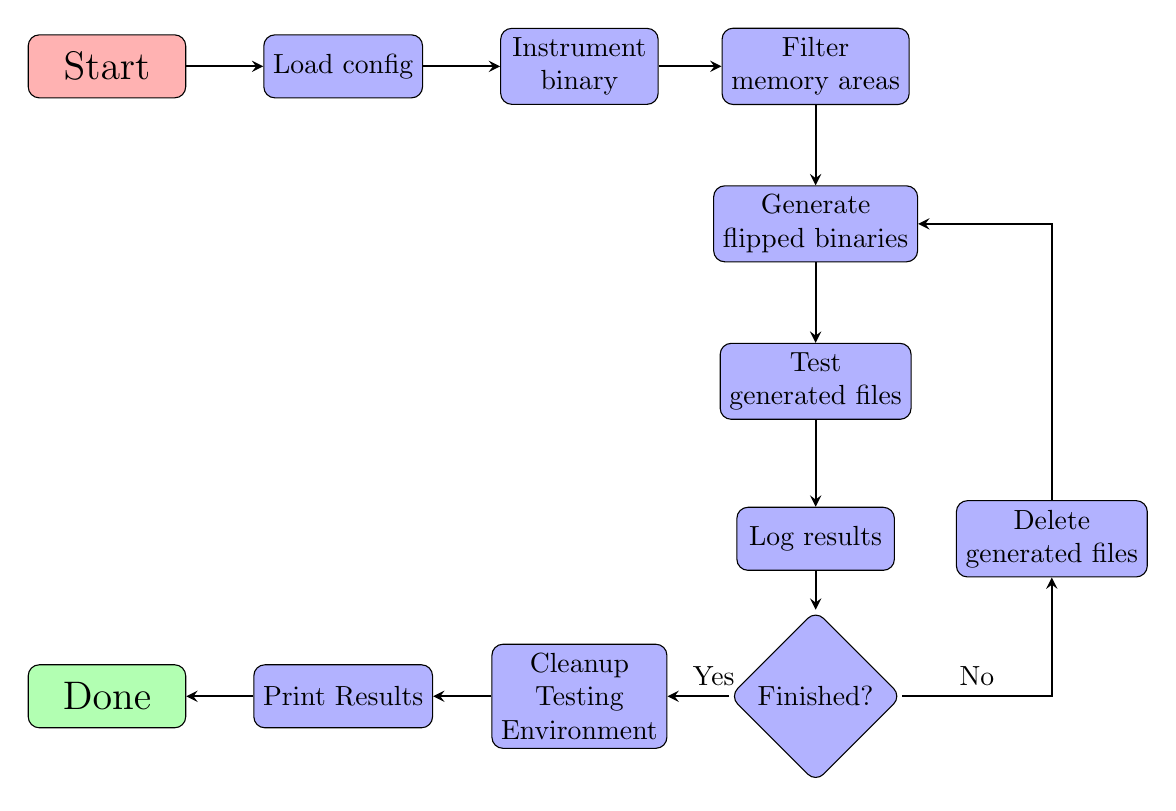
\begin{tikzpicture}
  % Nodes of the framework
  \node (start) [root] {Start};
  \node (conf) [function, right of=start, xshift=2cm] {Load config};
  \node (instr) [function, right of=conf, align=center, xshift=2cm]
                {Instrument \\ binary};
  \node (filter) [function, right of=instr, align=center, xshift=2cm]
                 {Filter \\ memory areas};
  \node (gen) [function, below of=filter, align=center, yshift=-1cm]
              {Generate \\ flipped binaries};
  \node (test) [function, below of=gen, align=center, yshift=-1cm]
               {Test \\ generated files};
  \node (report) [function, below of=test, align=center, yshift=-1cm]
                 {Log results};
  \node (clean) [function, right of=report, align=center, xshift=2cm]
                {Delete \\ generated files};
  \node (dec) [decision, below of=report, align=center, yshift=-1cm]
              {Finished?};
  \node (propclean) [function, left of=dec, align=center, xshift=-2cm]
                    {Cleanup \\ Testing \\ Environment};
  \node (printres) [function, left of=propclean, align=center, xshift=-2cm]
                   {Print Results};
  \node (finish) [finish, left of=printres, xshift=-2cm] {Done};
  % Connections
  \draw [arrow] (start) -- (conf);
  \draw [arrow] (conf) -- (instr);
  \draw [arrow] (instr) -- (filter);
  \draw [arrow] (filter) -- (gen);
  \draw [arrow] (gen) -- (test);
  \draw [arrow] (test) -- (report);
  \draw [arrow] (report) -- (dec);
  \draw [arrow] (dec) -- (propclean) node[near start, above] {Yes};
  \draw [arrow] (propclean) -- (printres);
  \draw [arrow] (printres) -- (finish);
  \draw [arrow] (dec) -| (clean) node[near start, above] {No};
  \draw [arrow] (clean) |- (gen);
  \end{tikzpicture}
  \caption{Flowchart showing each part of the framework and their connections.}
  \label{fig:frameworkdesign}
\end{figure}

We have implemented a framework to search for exploitable bitflips in programs.
Figure~\ref{fig:frameworkdesign} shows a diagram describing the
framework\textquotesingle s design. We split it into multiple parts:

\begin{enumerate}
\begin{samepage}
  \item Accessed memory areas are logged from all the ELF files the program
uses.
  \item Pre-defined filters are applied to the reported memory areas.
  \item ELF files for each of the bit flips are generated.
  \item Each ELF file gets executed, and the behaviour is checked against a
pre-defined success state
\end{samepage}
\end{enumerate}

\begin{figure}
\centering
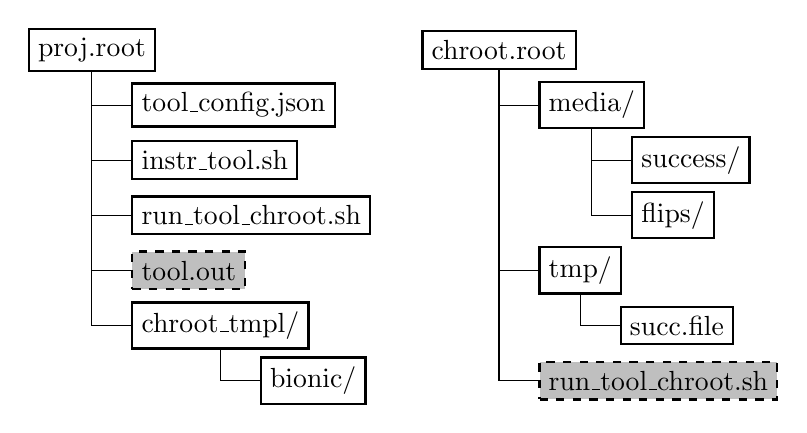
\begin{tikzpicture}[%
  grow via three points={one child at (0.5,-0.7) and
  two children at (0.5,-0.7) and (0.5,-1.4)},
  edge from parent path={(\tikzparentnode.south) |- (\tikzchildnode.west)}]
  \node [fsnode] {proj.root}
    child {node[fsnode] {tool\_config.json}}
    child {node [fsnode] {instr\_tool.sh}}
    child {node [fsnode] {run\_tool\_chroot.sh}}
    child {node [fsnode, optional] {tool.out}}
    child {node [fsnode] {chroot\_tmpl/}
      child {node [fsnode] {bionic/}}
      };
  \node [fsnode, xshift=5cm] {chroot.root}
    child {node [fsnode] {media/}
      child {node [fsnode] {success/}}
      child {node [fsnode] {flips/}}
    }
    child [missing] {}
    child [missing] {}
    child {node [fsnode] {tmp/}
      child {node [fsnode] {succ.file}}
    }
    child [missing] {}
    child {node [fsnode, optional] {run\_tool\_chroot.sh}};
\end{tikzpicture}
\caption{File system structure of the framework and the chroot loaded for the
test runs, whereas the chroot is created from a templated loaded from the
\texttt{proj.root} and the \texttt{run\_tool\_chroot.sh} is copied over to the
created chroot.}
\label{fig:framfilesys}
\end{figure}

Each part of the framework is designed to work on its own and has a clearly
defined in- and output-interface. The parts can be adopted or easily used for
other testing purposes. The configuration file for the framework defines how
each step is applied to the application, as instrumentation and verification may
differ for each program. The file in Listing~\ref{lst:expconfig} shows an
example configuration file for the framework. Figure~\ref{fig:framfilesys} shows
the layout of the framework in the file system. The configuration file tells the
framework where to find each of the required files. The template chroot
describes the system used for testing.

\begin{figure}
\begin{minipage}{\linewidth}
\begin{lstlisting}[style=nasm,
                   caption={JSON style config file for the framework, showing
all parameters used to tweak each part of the framework. Entries
starting with \texttt{CR\_} are used inside the testing \texttt{chroot}.},
                   label={lst:expconfig}]
{
  "instrumenter_call": "./instr_tool.sh",
  "instrumenter_outfile": "tool.out",
  "chroot_template": "chroot_tmpl/bionic",
  "tmp_chroot_folder": "/media/ramdisk/chroot/",
  "folder_with_flips": "/media/ramdisk/flips/",
  "num_of_parallel_checks": 1,
  "CR_exec_file": "./run_tool_chroot.sh",
  "CR_flip_folder": "/media/flips",
  "CR_success_folder": "/media/success/",
  "CR_log_file": "/tmp/succ.file"
}
\end{lstlisting}
\end{minipage}
\end{figure}

The framework starts with executing \texttt{instr\_tool.sh} to generate a report
showing all bitflips to test. Additionally, it can also filter them. After the
script\textquotesingle s execution, the \texttt{tool.out}-file contains a list
of all byte positions to flip and test. Afterwards, the defined number of
chroots are created by copying the template from \texttt{chroot\_tmpl}. The
flipped binaries are copied to each \texttt{/media/flips} folder in the testing
chroot. The \texttt{run\_tool\_chroot.sh} file is copied to each testing
environment and executed there. This script runs in each of the \texttt{chroot},
replaces the original binary with a flipped version, runs the configured program
and checks it\textquotesingle s outcome. If the outcome matches a pre-defined
success state, the flipped binary is stored and reported by the framework after
all test runs are finished.

\subsubsection{Instrumenting the Program}

\begin{figure}
\begin{minipage}{\linewidth}
\begin{lstlisting}[style=CStyle,
                   caption={Example C++ code for a pintool logging memory
accesses. The tool stores the locations of instructions and parameters if they
point to memory. The tool stores accesses for reading and writing seperately.},
                   label={lst:pinlogcode}]
ADDRINT ins_addr = INS_Address(ins);
IMG img = IMG_FindByAddress(ins_addr);
ADDRINT base = IMG_LowAddress(img);
img_offsets[base] = IMG_LoadOffset(img);

for(size_t i = 0; i < INS_Size(ins); i++)
  accesses.insert(std::make_pair(ins_addr + i, base));

UINT32 memOperands = INS_MemoryOperandCount(ins);
for (UINT32 memOp = 0; memOp < memOperands; memOp++)
{
  if(INS_MemoryOperandIsRead(ins, memOp))
  {
    INS_InsertPredicatedCall(
      ins, IPOINT_BEFORE, (AFUNPTR)RecordMemRead,
      IARG_INST_PTR,
      IARG_MEMORYREAD_EA,
      IARG_ADDRINT, base,
      IARG_MEMORYREAD_SIZE,
      IARG_END);
  }
  if(INS_MemoryOperandIsWritten(ins, memOp))
  {
    INS_InsertPredicatedCall(
      ins, IPOINT_BEFORE, (AFUNPTR)RecordMemWrite,
      IARG_INST_PTR,
      IARG_MEMORYWRITE_EA,
      IARG_ADDRINT, base,
      IARG_MEMORYWRITE_SIZE,
      IARG_END);
  }
}
\end{lstlisting}
\end{minipage}
\end{figure}

We use Intel Pin~\cite{pintool} for instrumentation. We log every memory access
during execution of the program. We want to log all accesses which happen inside
of ELF files, which means the program\textquotesingle s binary and all libraries
it uses during runtime. The pintool we use to achieve this, adds instrumenter
calls to all memory accesses. The tool then logs all accesses per binary and the
offsets of the address in the corresponding ELF file. This information is
required to determine which accessed area is mapped to which file later on.

Listing~\ref{lst:pinlogcode} shows a code snippet of the used pintool which
logs all memory accesses as it instruments each instruction and logs the opcode
position and its parameters if they address memory. For Pin, the
image~\texttt{img} refers to an ELF file stored on the hard drive, the images
represent the program\textquotesingle executable and the dynamic libraries
loaded during execution. The \texttt{INS\_InsertPredicatedCall} function is used
to insert a function call on the machine code layer. The function can have an
arbitrary number of parameters, as the user has to define the function with each
parameter and type. Pin then inserts a call to the given function pointer and
manages the handling of the parameters and return values in a way that the
instrumented program\textquotesingle s execution is not affected.

We instrument the program with a run resulting in a failed state, after the run,
we filter the accessed memory areas for each file and check if areas were
written before reading. If so, we can also skip testing those bits, as the
program would overwrite the flips again.

Instrumentation is done via the configured \texttt{instrumenter\_call} in the
config file shown in Listing~\ref{lst:expconfig}. The
\texttt{instrumenter\_call} generates the configured
\texttt{instrumenter\_outfile}. The output file contains the memory accesses
formated in the following manner:

\mbox{\texttt{<hex:position\_in\_file> - str:filename}}.

\subsubsection{Generating and Testing the Flips}

Next, we create a new ELF file for each bit for each of the reported bytes.
Depending on the configured number of parallel checks, chroots are created. The
framework makes sure the number of created ELF files does not require more than
the memory available. If there are more files to test than the available memory
allows, the framework takes multiple runs, as shown in
Figure~\ref{fig:frameworkdesign}. A test run starts configured
\texttt{CR\_exec\_file} which will copy a flipped file from the
\texttt{CR\_flip\_folder} to the original position, then run it and check if the
output matches a defined success state. If the flipped file reaches the success
state, the framework writes the flipped address to the \texttt{CR\_log\_file}
and copies the flipped ELF file to the \texttt{CR\_success\_folder}. The
framework passes the file to replace to the \texttt{CR\_exec\_file} when it
calls it. To keep track of which bitflip is tested the filename for generated
ELF files is structured as follows:

\mbox{\texttt{<original\_filename>\_<address\_in\_file>\_<bit\_number>}}.

\subsection{Tweaks added to the Framework}

As our framework reports all accessed memory areas, we apply some tweaks to
these reported memory areas generated with Pin. The additions help us to either
filter unnecessary flips and also to add memory areas which would be missed by
instrumentation as they are only accessed during the setup phase of the program.

\subsubsection{Filtering Memory Accesses}

As seen in Listing~\ref{lst:pinlogcode} we log accesses separated by reading and
writing. This separation is done to apply a simple filter on the reported memory
areas. It is not practical to test a memory area which is written before being
read, as the program will overwrite the memory area before a bitflip would
influence the execution path. We, therefore, test memory areas which are either
only read or read before write access.

\subsubsection{Testing flips in the ELF structure}

As described in Section~\ref{sec:elf}, the ELF structure contains information
for the linker on where to load different segments of the binary in the virtual
address space. Applying flips in this section could lead to misplaced libraries
or different offsets for segment mappings. A call of a function might result in
executing different code as intended and lead to a different outcome of the
program. Therefore, we also test each bit which is used for representing ELF
structures.

\subsubsection{Instrumenting Binaries running as superuser}
~\label{sec:setuidfix}

Some binaries behave differently when being run by a superuser. For example
\texttt{sudo} is a \texttt{setuid} binary owned by \texttt{root}, therefore the
active user running the binary is \texttt{root}. If Pin is running as a regular
user, it is not allowed to access the memory of a superuser\textquotesingle s
process, it, therefore, cannot instrument \texttt{sudo}. Running Pin as
superuser is possible, but starting \texttt{sudo} as \texttt{root} does not
trigger any authentication checks, as the calling user already got superuser
permissions, therefore a change of the current user is not required.

We use the attach-to-process functionality of Pin to bypass this behaviour. In
that way, we can start \texttt{sudo} as a regular user and run Pin as superuser.
We would start \texttt{sudo} and then attach to the resulting process ID. The
problem here is that getting the process ID takes time and during that time
\texttt{sudo} could already perform accesses which then would be missed by
instrumentation. Therefore, we preload a shared library which keeps the
\texttt{sudo} program in a defined state for some time to give the framework
enough time to look up the ID and instrument all relevant code parts.

\begin{figure}
\begin{minipage}{\linewidth}
\begin{lstlisting}[style=CStyle,
                   caption={Code of the preloaded library to keep the process
waiting for some milliseconds, which gives enough time for Pin to attach to the
process.},
label=lst:presleeplib]
extern const char *__progname;

__attribute__((constructor)) void init(void)
{
  if(!strcmp(__progname, "instrumented_program"))
  {
    size_t i = 0;
    while(i++ < 600000000);
  }
}
\end{lstlisting}
\end{minipage}
\end{figure}

Listing~\ref{lst:presleeplib} shows the code used to generate such a preloaded
library. We use the counting while-loop instead of a call to the sleep system
call because attaching Pin to a process in sleeping state results in a state
where the process cannot wake up again. We also experienced the same issue with
debugging tools on our Linux-based environment, such as \texttt{gdb}. The number
of increments was chosen to have enough time to search the process ID and attach
to it. The compiler attribute \texttt{constructor} makes sure the program
executes this code on loading the library before any other code. We add the path
to our library to the \texttt{/etc/ld.so.preload} file, which makes sure the
library is preloaded by any executed program. The name of the executable is
checked in Line 5 of Listing~\ref{lst:presleeplib} to only call the while-loop
when the binary is our instrumentation target. Otherwise, all executed programs
would execute the time-consuming while-loop during startup.

\subsection{Comparing our Approach to other Techniques}

Our described approach for finding exploitable bitflips is built on a
fuzzing-like approach. We want to look at other ideas we tried to adapt or use
for the searching and argument on why we stuck with our described framework.

\subsubsection{Symbolic Execution}

\texttt{angr}~\cite{angrpaper} offers many tools and functions for binary
analysis and symbolic execution. For this, it can load a binary, search all
possible states and provides locations in the executable where a state has more
than one possible successor. \texttt{angr} allows searching for inputs and
arguments which would end up in a state defined as successful. This state could
either be defined by an address reached during execution or on the output of the
program. The approach \texttt{angr} seems useful for our task of searching
bitflips to change to a success state. However, \texttt{angr} is very limited
when changing the executed machine code to find new states. It works well for
finding inputs for the program to result in a success state. Testing bitflips
with \texttt{angr} results in a limited application of the tool\textquotesingle
s possibilities, where the binary is loaded, a bitflip is applied, and a single
run is made which is then checked if it ends up in the defined success state.
Changing inputs or arguments will not be tested. \texttt{angr} could be used to
test bitflips, but the time needed would be about \SI{10} to \SI{15} times
larger than our approach, because of the time it takes \texttt{angr} to load and
the program and its libraries.

\subsubsection{Using AFL}

Fuzzers like AFL~\cite{aflweb} tests a program by applying different forms of
input and generate those applying a form of edge coverage to learn from changes
from the control flow. AFL uses instrumentation to document the
program\textquotesingle s control flow and adapt its test cases based on changes
of it. AFL offers source code based instrumentation, which might not be suitable
for testing bitflips in binaries as with that approach, the tested executables
would change. According to their documentation~\cite{aflreadme}, AFL also offers
instrumentation of binary-only application. Here they use the QEMU processor
emulator~\cite{qemuweb} as a userland virtual machine. They state in Section 4
of the documentation~\cite{aflreadme} that in this mode execution is 2-5 times
slower than for the compile-time instrumentation approach.

For testing bitflips, the adaption of test cases can be ignored, as we always
stick to the same environment and external inputs. The AFL techniques to learn
from control flow changes could be adapted but as we do not want to build on
source-based instrumentation because of binary changes the additional execution
time for their binary instrumentation made the AFL adaption not practical.

\subsubsection{Using a Fuzzing-like Approach}

The described instrumentation based fuzzing of AFL can be adapted for
instrumentation based bitflip testing. We used Intel Pin~\cite{pintool} for this
approach, as it is the best performing tool for binary instrumentation. The
implementation would instrument every instruction of the program, fork multiple
times. One time for each bit in the instruction and the addressed memory by the
instruction. After the forks, individual bitflips are applied to the memory of
the new processes, and the new processes continue execution without
instrumentation. The outputs of the new processes are then checked for resulting
in a successful state.

This approach turned out to be practical and performed well enough for simple
programs. However, we ran into problems with applications which had the
\texttt{setuid} property and the solution we described in
Section~\ref{setuidfix} did not work for this time. Looking at the execution
times for simple programs they were just a little lower, about \SI{5}{\percent}
as for running pre-generated binary files. However, the time needed for the
generation would be saved, and the memory footprint would be lower as the
processes memory would be copy-on-write. We decided to not go with this
approach, as we wanted to test all kind of binaries, also \texttt{setuid} ones,
such as \texttt{sudo}.

For our framework, we generated the binaries containing the bitflip still in
DRAM memory, to speed up the procedure of copying and applying a bitflip. This
generation phase of the framework showed to take less than \SI{1}{\percent} of
the whole testing process time. Therefore, running multiple generation phases,
because of the increased memory usage, was accepted as a downside of our chosen
testing approach.

%%%%%%%%%%%%%%%%%%%%%%%%%%%%%%%%%%%%%%%%%%%%%%%%%%%%%%%%%%%%%%%%%%%%%%%%%%%%%%%%

\chapter{Case Study: Rowhammer-targets in real-world Applications}
\label{sec:results}

In this thesis, we want to apply the framework to larger, real-world
applications, with realistic bitflip targets. As
Gruss~\etal~\cite{flipinthewall} already showed, there are bits in the
\texttt{sudoers} library which, when toggled, allow using \texttt{sudo} without
or with a wrong password to still gain the privileges of a superuser. We show
that our framework can find a larger number of exploitable bitflips. We present
the results of the framework applied to real-world applications, which are
commonly used in Linux-based operating systems. In this section, we present all
the applications we tested, the pre-defined successful outcomes, and the
bitflips leading to the desired behaviour. For the results, we discuss how many
exploitable bitflips were found, in what memory section they were and if in an
instruction, in which part. In the end, we want to give some statistic about the
exploitable bitflips and also point out the ones which were exploitable in
multiple applications.

For testing, we used a \texttt{Debian GNU/Linux 9.5} operating system. The
testing environment inside the \texttt{chroot} had the same system. The CPU used
was a \mbox{\texttt{Intel(R) Core(TM) i7-960}} and a total of
\SI{16}{\giga\byte} DRAM memory was installed.

\section{\texttt{sudo} - Privilege Escalation}

\texttt{sudo} is a tool used for privilege management on Linux-based operating
systems. Users can use it to execute commands as another user, if the
tool\textquotesingle s configuration allows it, also as the superuser
\texttt{root}. For the tool to run the given command as another user, the user
has to provide their password.

We want to find all exploitable flips which would allow a user to run
\texttt{sudo} without knowing the password. This exploit would result in a
privilege escalation as the user can become superuser with a bypass of the
credential check.

For testing we call \texttt{sudo} and provide a wrong password for the
credential check. As command we provide reading a file which is owned by
\texttt{root} and can not be read by the calling user. We define the success
state as the call of \texttt{sudo} must print the content of the file owned by
the superuser. We tested version $1.8.19p1$ of \texttt{sudo}.

\addtocontents{toc}{\protect\setcounter{tocdepth}{1}}
\subsection{Results}
\addtocontents{toc}{\protect\setcounter{tocdepth}{2}}

\begin{table}[!htb]
\centering
\begin{tabular}{c|cccc|c}
ELF File & \texttt{.text}  & \texttt{.rodata} & \texttt{.got.plt} &
\texttt{.plt} & Sum of flips:                             \\ \hline
\texttt{ld-linux-x86-64.so.2} & 1   & 0  & 0  & 0  & 1    \\
\texttt{libpthread.so.0}      & 2   & 0  & 0  & 0  & 2    \\
\texttt{sudo}                 & 6   & 0  & 0  & 0  & 6    \\
\texttt{libnns\_compat.so.2}  & 6   & 0  & 1  & 0  & 7    \\
\texttt{libpam.so.0}          & 64  & 0  & 0  & 0  & 64   \\
\texttt{pam\_unix.so}         & 85  & 0  & 0  & 1  & 86   \\
\texttt{sudoers.so}           & 219 & 35 & 5  & 0  & 259  \\ \hline
Sum of flips:                 & 383 & 35 & 6  & 1  & 425
\end{tabular}
\caption{List of ELF files used by the \texttt{sudo(1.8.19p1)} program and the
number of flips causing privilege escalation listed per section.}
\label{tab:sudores}
\end{table}

We present \SI{425} exploitable bitflips in total. Table~\ref{tab:sudores} shows
the ELF files where the flips were found and also shows how many bitflips were
exploitable in different ELF sections.  Most bitflips were found in the
\texttt{sudoers} library but also bits in the linker
(\texttt{ld-linux-x86-64.so.2}) and the threading library
(\texttt{libpthread.so.0}) were exploitable.

We can see that most exploitable bitflips are in the \texttt{.text} sections of
binaries, which is the section holding the executed machine code. The
\texttt{.plt} section refers to the Procedure Linkage Table, which is used to
resolve mappings between position-independent functions and their absolute
addresses. Close to the same is the \texttt{.got.plt} section, which represents
the global offset table, which resolves mappings for position-independent code
parts.

\begin{table}[!htb]
\centering
\begin{tabular}{c|cc|c}
ELF File & opcode & parameter & Sum of flips: \\ \hline
\texttt{ld-linux-x86-64.so.2} & 0 & 1  & 1    \\
\texttt{libpthread.so.0}      & 0 & 2  & 2    \\
\texttt{sudo}                 & 2 & 4  & 6    \\
\texttt{libnns\_compat.so.2}  & 2 & 5  & 7    \\
\texttt{libpam.so.0}          & 17 & 47   & 64   \\
\texttt{pam\_unix.so}         & 36 & 50   & 86   \\
\texttt{sudoers.so}           & 87 & 172  & 259  \\ \hline
Sum of flips:                 & 144 & 281 & 425
\end{tabular}
\caption{List of bitflips causing privilege escalation in
\texttt{sudo(1.8.19p1)} and what they change in instructions.}
\label{tab:sudoflip}
\end{table}

From the \SI{425} exploitable flips \SI{144} were placed in the opcodes of
instructions and \SI{281} were in parameters. Table~\ref{tab:sudoflip} shows how
the flips are divided in that two section for the different ELF files. It is
shown for all files. That about one-third of the flips are applied in the
opcodes and the other two in the parameters.

\begin{figure}
\begin{minipage}{\linewidth}
\begin{lstlisting}[style=diff,
                   caption={Diff for a bitflip applied to
\texttt{libnss\_compat.so.2} in order to bypass a user privilege check. The call
to \texttt{strcmp} is exchanged because the offset used for the lookuptable
is flipped.},
label=lst:sudoex]
  351b:  0f 84 90 00 00 00  je     35b1
  3521:  48 89 ee           mov    %rbp,%rsi
- 3524:  e8 47 dc ff ff     callq  1170 <strcmp@plt>
+ 3524:  e8 c7 dc ff ff     callq  11f0 <malloc@plt>
  3529:  85 c0              test   %eax,%eax
  352b:  0f 85 3e ff ff ff  jne    346f
\end{lstlisting}
\end{minipage}
\end{figure}

Listing~\ref{lst:sudoex} shows a diff of the \texttt{libnss\_compat.so.2} ELF
file, where a call to \texttt{strcmp} is replaced with a call to \texttt{malloc}
by a single bitflip, causing the later \texttt{jne} instruction to behave
differently.

Testing the \texttt{sudo} program for exploitable bitflips took about \SI{8}
hours of CPU time. The testing was parallelised and split into 24
\texttt{chroot} environments. Testing all bits in the \texttt{sudo} binary
itself took about two to three times as long in an equal configuration.

\section{\texttt{nginx} - HTTP Basic Authentication Bypass}

\texttt{nginx} is a web server, available on for Linux-based operating
systems.~\cite{nginxweb}. The tool can be used to serve websites, and it can
also be configured to support basic authentication schemes.

We want to find all exploitable bitflips which would allow an attacker to access
websites protected with HTTP basic authentication. Such an exploit would bypass
the credential check of the configured web server, which uses \texttt{htpasswd}
for the basic authentication, as described in Section~\ref{sec:httauth}.

For testing we start \texttt{nginx}, wait for about \SI{100}{\milli\second} for
the server to go into an initialised state. Then we request a website protected
with HTTP basic authentication, providing credentials containing the correct
username but a wrong password. If the response contains the content of the
requested website, we add the flipped bit to the list of exploitable bitflips.
We do not care if the response is malformed. We rate the response as successful
as long as the protected site is leaked by it. We tested version $1.10.4$ of
\texttt{nginx}.

\addtocontents{toc}{\protect\setcounter{tocdepth}{1}}
\subsection{Results}
\addtocontents{toc}{\protect\setcounter{tocdepth}{2}}

For the authentication bypass in \texttt{nginx} we can report that only bitflips
in the program\textquotesingle s binary itself were exploitable. We can show
\SI{298} exploitable bitflips in the executable, where all of them were found in
the \texttt{.text} section of the ELF file.

\begin{figure}
\begin{minipage}{\linewidth}
\begin{lstlisting}[style=diff,
                   caption={Diff of the disassembly for a bitflip applied to
the \texttt{nginx} binary in order to bypass the credential check. The
\texttt{add} instruction is prefixed with a \texttt{0x40}, which is the Intel
REX prefix used to change addressing modes. This prefix changes the computation
before the jump to \texttt{ngx\_http\_headers\_out} at address
\texttt{0x2f1399}.},
label=lst:nginxex]
  2f1365:  00 00                 add    %al,(%rax)
  2f1367:  00 91 7a 0c 00 00     add    %dl,0xc7a(%rcx)
  2f136d:  00 00                 add    %al,(%rax)
  2f136f:  00 10                 add    %dl,(%rax)
- 2f1371:  00 00                 add    %al,(%rax)
- 2f1373:  00 00                 add    %al,(%rax)
- 2f1375:  00 00                 add    %al,(%rax)
- 2f1377:  00 a1 7a 0c 00 00     add    %ah,0xc7a(%rcx)
- 2f137d:  00 00                 add    %al,(%rax)
- 2f137f:  00 14 00              add    %dl,(%rax,%rax,1)
- 2f1382:  00 00                 add    %al,(%rax)
- 2f1384:  00 00                 add    %al,(%rax)
- 2f1386:  00 00                 add    %al,(%rax)
- 2f1388:  b2 7a                 mov    $0x7a,%dl
- 2f138a:  0c 00                 or     $0x0,%al
- 2f138c:  00 00                 add    %al,(%rax)
- 2f138e:  00 00                 add    %al,(%rax)
- 2f1390:  0d 00 00 00 00        or     $0x0,%eax
+ 2f1371:  40 00 00              add    %al,(%rax)
+ 2f1374:  00 00                 add    %al,(%rax)
+ 2f1376:  00 00                 add    %al,(%rax)
+ 2f1378:  a1 7a 0c 00 00 00 00  movabs 0x1400000000000c7a,%eax
+ 2f137f:  00 14
+ 2f1381:  00 00                 add    %al,(%rax)
+ 2f1383:  00 00                 add    %al,(%rax)
+ 2f1385:  00 00                 add    %al,(%rax)
+ 2f1387:  00 b2 7a 0c 00 00     add    %dh,0xc7a(%rdx)
+ 2f138d:  00 00                 add    %al,(%rax)
+ 2f138f:  00 0d 00 00 00 00     add    %cl,0x0(%rip)  <ngx_http_headers_out>
  2f1395:  00 00                 add    %al,(%rax)
  2f1397:  00 c7                 add    %al,%bh
  2f1399:  7a 0c                 jp     2f13a7  <ngx_http_headers_out>
  2f139b:  00 00                 add    %al,(%rax)
\end{lstlisting}
\end{minipage}
\end{figure}

\SI{65} bitflips changed the opcode of an instruction \SI{231} changed
parameters. \SI{2} bitflips changed the context of the executable memory area
because the instruction length was changed by the flip and therefore the context
was changed. In Listing~\ref{lst:nginxex} we can see how changing the lenght of
the \texttt{add} instruction can result in a different outcome for the
execution.

Testing the \texttt{nginx} ELF files took a total of about \SI{18}{\hour} CPU
time. The timing is that high, because we had to make sure the server is up and
ready to reply to our requests for each test. For testing, we have used eight
parallel testing-\texttt{chroot} instances.

\section{\texttt{sshd} - Secure Shell Server Login Bypass}

\texttt{sshd} is a secure shell server implementation which runs on Linux-based
operating systems. It is used together with the \texttt{ssh} client, which
allows to log in on remote hosts via the \texttt{ssh} protocol. According to the
documentation~\cite{sshman}, not only log in via username and password
credentials is supported, but also public key cryptography can be used for
authentication.

We want to find all exploitable bitflips which would allow an attacker to log
into a remote machine without knowing the correct password of the user. The
\texttt{ssh} server is configured to allow accesses from users using password
authentication.

For testing, we start \texttt{sshd}, wait for \SI{100}{\milli\second} for the
server to start and be ready to accept connections. We then use a \texttt{ssh}
client to execute commands in the testing environment via the secure shell
connection. We defined a success state when the output of the client showed a
successful login. We verified the login by executing \texttt{whoami}, which
returns the name of the logged in user. We tested version $7.4p1$ of the
\texttt{ssh} server.

\addtocontents{toc}{\protect\setcounter{tocdepth}{1}}
\subsection{Results}
\addtocontents{toc}{\protect\setcounter{tocdepth}{2}}

For the used \texttt{ssh} server we can only report working bitflips in the
loaded libraries. Additional, all of the reported flips were found in the
\texttt{.text} section of the ELF files. Table~\ref{tab:sshdres} gives an
overview of the number of flips found per file. We can see, that most bitflips
can be found in the \texttt{libc} of the host system, also the cryptographic
library and the linker are affected for Rowhammer targeting a \texttt{ssh}
login.

\begin{table}[!htb]
\centering
\begin{tabular}{c|c}
ELF File               & \texttt{.text} \\ \hline
\texttt{libc.so.6}         & $34$ \\
\texttt{libcrypto.so.1.0.2} & $6$ \\
\texttt{ld-linux-x86-64.so.2} & $1$ \\ \hline
Sum of flips:                 & $41$
\end{tabular}
\caption{List of flips inside the \texttt{sshd(7.4p1)} program
causing a authentication bypass, whereas all of them were in the \texttt{.text}
sections of dynamically loaded libraries.}
\label{tab:sshdres}
\end{table}

\begin{figure}
\begin{minipage}{\linewidth}
\begin{lstlisting}[style=diff,
                   caption={Diff for a bitflip applied to the
\texttt{libcrypto.so.1.0.2} binary in order to bypass a credential check. The
move from \texttt{rbx} to \texttt{rdi} is exchanged with a move to
\texttt{r15}, this changes the parameter for \texttt{EVP\_MD\_CTX\_test\_flags},
which is highly likely to result in a different outcome.},
label=lst:sshdex]
   1341c5:      74 ad                  je     134174 <EVP_MD_CTX_cleanup>
   1341c7:      be 04 00 00 00         mov    $0x4,%esi
-  1341cc:      49 89 df               mov    %rbx,%rdi
+  1341cc:      48 89 df               mov    %rbx,%r15
   1341cf:      e8 dc e5 f3 ff         callq  727b0 <EVP_MD_CTX_test_flags@plt>
   1341d4:      85 c0                  test   %eax,%eax
\end{lstlisting}
\end{minipage}
\end{figure}

In Listing~\ref{lst:sshdex}, we show a diff for the \texttt{libcrypto} library
used by \texttt{ssh}. We can see how changing the function parameters
(\texttt{rdi}) for \texttt{EVP\_MD\_CTX\_test\_flags@plt} changes the outcome
of the libary call in a way ssh will think it is working with correct
credentials.

Testing the \texttt{ssh} server took about six hours. The timing here is lower
than for \texttt{nginx} or \texttt{sudo}, as the shell server was faster ready
than \texttt{nginx}, and there were not so many flips to test as in
\texttt{sudo}.

\section{Local Login Bypass on Linux-based Operating Systems}

If attackers have local access to computers and the network, the nethammer
attack~\cite{nethammer} could be used to introduce bitflips to the running
system. An attacker could target the login procedure to gain full access to the
system. On most Linux-based systems local logins are done via the
\texttt{/bin/login} application. This program is called on the default terminal
by the init process, after the bootup of the operating system. The goal is to
find bitflips which would allow logging in without knowing the correct password.

\addtocontents{toc}{\protect\setcounter{tocdepth}{1}}
\subsection{Instrumentation}
\addtocontents{toc}{\protect\setcounter{tocdepth}{2}}

As the \texttt{/bin/login} binary has to be run as root, we use a similar
approach as for \texttt{sudo}. We again make use of the preloaded library from
Listing~\ref{lst:presleeplib}. The instrumentation for \texttt{/bin/login} takes
longer than for the other programs. A reason for this could either be the key
derivation functions used or timeouts build in to prevent brute-forcing the
local login. We start the program and attach to the created process shortly
after, we then try to login with a wrong password and wait for the application
to quit. All accesses during this are logged. To simplify the procedure, we
configure the login to allow just one login try instead of the default five.

\addtocontents{toc}{\protect\setcounter{tocdepth}{1}}
\subsection{Testing}
\addtocontents{toc}{\protect\setcounter{tocdepth}{2}}

\texttt{/bin/login} expects input on a \texttt{TTY}, the Linux terminal
interface, using pipes to redirect the input does not work for testing. To get
around this issue, we use \texttt{passh}~\cite{passhweb}, which is usually used
for automating \texttt{ssh} logins, but it also works for our problem. To find
out if we result in a successful state, we run the login binary as root, send
credentials with a correct username and a wrong password, and check if the
system changed the current user from \texttt{root} to the other user. We tested
the \texttt{/bin/login} binary included in the \texttt{shadow-utils 4.4}.

\addtocontents{toc}{\protect\setcounter{tocdepth}{1}}
\subsection{Results}
\addtocontents{toc}{\protect\setcounter{tocdepth}{2}}

For \texttt{/bin/login}, we can report bitflips in loaded libraries and also the
program\textquotesingle s binary itself. All the found bitflips were in the
\texttt{.text} section of ELF files. As Table~\ref{tab:loginres} shows, there
were $178$ flips ending in a successful bypass of the login service. Most flips
were found in \texttt{pam} libraries, which are a major part of the user
management in Linux-based operating systems.

\begin{table}[!htb]
\centering
\begin{tabular}{c|c}
ELF File               & \texttt{.text} \\ \hline
\texttt{login}         & $57$ \\
\texttt{pam\_unix.so} & $64$ \\
\texttt{pam\_nologin.so} & $2$ \\
\texttt{pam\_securetty.so} & $5$ \\
\texttt{libpam.so.0} & $50$ \\ \hline
Sum of flips:                 & $178$
\end{tabular}
\caption{List of flips inside the \texttt{login(shadow-utils 4.4)} program
causing a bypass of the local login check.}
\label{tab:loginres}
\end{table}

\begin{figure}
\begin{minipage}{\linewidth}
\begin{lstlisting}[style=diff,
                   caption={Diff for a bitflip applied to the
\texttt{pam\_nologin.so} binary in order to bypass a credential check. The
pop to register $15$ gets exchanged with a pop to register $14$, therefore the
value of \texttt{r15} and \texttt{r14} are not as desired and hence the
execution path of \texttt{/bin/login} changes in a way the login
procedure succeeds.},
label=lst:loginex]
  c37:  41 5d                   pop    %r13
  c39:  41 5e                   pop    %r14
- c3b:  41 5f                   pop    %r15
+ c3b:  41 5e                   pop    %r14
  c3d:  c3                      retq
  c3e:  66 90                   xchg   %ax,%ax
\end{lstlisting}
\end{minipage}
\end{figure}

In Listing~\ref{lst:loginex}, we show a diff for the \texttt{pam\_nologin.so}
file after a bitflip was applied at the address \texttt{0x0c3b}. With
the applied flip, register values get changed as the value which should be
written to register $15$ is placed in register $14$ instead, overwriting the
value placed there before.

Testing \texttt{/bin/login} tool about 35 hours. This is mainly due to the long
response time by the program itself, which is probably a countermeasure against
local brute-forcing. Also, there were by far the most memory accesses reported
by the instrumentation pintool.

\section{Summery of the Results}

In summary, we can show, that all our tested programs can be exploited by
bitflips. We show that Rowhammer can be used for privilege escalation and
security bypasses in common applications used in most Linux-based operating
systems. We can report that most bitflips can be found in the \texttt{.text}
section of ELF files, which contains the executed machine code. Also, we show
that not only binaries on its own are suffering such flaws, but also loaded
libraries introduce exploitable bitflips to programs. The diffs of the
disassembly show, that when flipping code, not only the opcode can be abused but
also parameters in instructions.

\begin{table}[!htb]
\centering
\begin{tabular}{c|c}
ELF File               & Shared flips \\ \hline
\texttt{pam\_unix.so} & $52$ \\
\texttt{libpam.so.0} & $18$ \\ \hline
Sum of flips:                 & $70$
\end{tabular}
\caption{Number of flips which work for a login bypass and a \text{sudo}
privilege escalation.}
\label{tab:loginsudo}
\end{table}

Besides that, we can report that some bitflips cause a bypass in multiple
application. For example most \texttt{pam} related flips can be abused in the
\texttt{login} program and \texttt{sudo} as both check against the same user
management. An attacker, therefore, could introduce a flip in the
\texttt{libpam.so.0} file, log in as the user and gain super-user access if the
user is allowed to use \texttt{sudo}. Table~\ref{tab:loginsudo} show the exact
number of shared bitflips between the two applications. Also, for \texttt{sudo}
and \texttt{sshd}, there was one shared bitflip found, namely one in the
\texttt{ld-linux-x86-64.so.2} file at address \texttt{0xfc6c}.
%}}}

%% vim:foldmethod=expr
%% vim:fde=getline(v\:lnum)=~'^%%%%\ .\\+'?'>1'\:'='
%%% Local Variables:
%%% mode: latex
%%% mode: auto-fill
%%% mode: flyspell
%%% eval: (ispell-change-dictionary "en_US")
%%% TeX-master: "main"
%%% End:

%%%%%% Dynamic Data Attack %%%%%%%%%%%%%%%%%%%%%%%%%%%%%%%%%%%%%%%%%%%%%%%%%%{{{
\chapter{Bitflip Attacks on Dynamic Data}\label{sec:dynattack}

In this chapter, we take a look at data created at the runtime of a program
and how bitflips applied to that memory could benefit an attacker. We will go
into details about OpenSSL and how bitflips can enable for instance
nonce-misuse attacks. We want to apply a similar attack as Böck~\etal~describe
in their work about ``practical nonce misusage attacks''~\cite{gcmnonceattack}.
By this, we want to show how Rowhammer can introduce new attack vectors to
applications.

\section{Analysis of OpenSSL for possible Nonce Misuse Flips}

\begin{figure}
\begin{minipage}{\linewidth}
\begin{lstlisting}[style=CStyle,
                   caption={Struct used by OpenSSL to describe the AES-GCM
context. The IV used is stored in the memory pointed to by \texttt{iv}. Source
is taken from OpenSSL version $1.1.0g$},
                   label={lst:aesstruct}]
typedef struct {
  union {
    double align;
    AES_KEY ks;
  } ks;                       /* AES key schedule to use */
  int key_set;                /* Set if key initialised */
  int iv_set;                 /* Set if an iv is set */
  GCM128_CONTEXT gcm;
  unsigned char *iv;          /* Temporary IV store */
  int ivlen;                  /* IV length */
  int taglen;
  int iv_gen;                 /* It is OK to generate IVs */
  int tls_aad_len;            /* TLS AAD length */
  ctr128_f ctr;
} EVP_AES_GCM_CTX;
\end{lstlisting}
\end{minipage}
\end{figure}

\begin{figure}
\begin{minipage}{\linewidth}
\begin{lstlisting}[style=CStyle,
                   caption={Context struct describing the Cipher used in TLS.
This struct is used as the SSL context inside OpenSSL. Source is taken from
OpenSSL version $1.1.0g$},
                   label={lst:ciphctx}]
struct evp_cipher_ctx_st {
  const EVP_CIPHER *cipher;
  ENGINE *engine;     /* functional reference if
                       * 'cipher' is ENGINE-provided */
  int encrypt;        /* encrypt or decrypt */
  int buf_len;        /* number we have left */
  unsigned char oiv[EVP_MAX_IV_LENGTH]; /* original iv */
  unsigned char iv[EVP_MAX_IV_LENGTH]; /* working iv */
  unsigned char buf[EVP_MAX_BLOCK_LENGTH]; /* saved partial
                                            * block */
  int num;           /* used by cfb/ofb/ctr mode */
  /* FIXME: Should this even exist? It appears unused */
  void *app_data;    /* application stuff */
  int key_len;       /* May change for variable length cipher */
  unsigned long flags; /* Various flags */
  void *cipher_data; /* per EVP data */
  int final_used;
  int block_mask;
  unsigned char final[EVP_MAX_BLOCK_LENGTH]; /* possible final
                                              * block */
} /* EVP_CIPHER_CTX */ ;
\end{lstlisting}
\end{minipage}
\end{figure}

We look at the implementation of AES-GCM inside OpenSSL. We see the general
AES-GCM context struct in Listing~\ref{lst:aesstruct}. Additional to that, we
take a look at the cypher-context struct in Listing~\ref{lst:ciphctx}. The
connection between those two is the initialisation vector \texttt{iv} which is
updated on each call of the GCM function.

To apply the described attack by Böck~\etal~\cite{gcmnonceattack}, we require
the \texttt{iv} to be reused by multiple GCM calls. OpenSSL uses a counter for
the \texttt{iv} for AES-GCM instead of a random value, flipping a bit to zero in
the \texttt{iv} causes a decrement of the counter which makes reuse likely. The
counter starts at a random value and is increased after. Therefore, a flip in
the lower bits is more likely to result in reuse of the nonce.
Böck~\etal~\cite{gcmnonceattack} state that this reuse constitutes breakage of
the cryptography for future messages and the attacker can craft valid
ciphertexts and overtake sessions. For the attack with Rowhammer, we target the
\texttt{iv} array in the \texttt{EVP\_CIPHER\_CTX} struct, as seen in
Listing~\ref{lst:ciphctx}.

\subsection{Likelihood of a Nonce-Misuse introduced by Rowhammer}

Lipp~\etal~\cite{nethammer} show that it is possible to send network requests
which cause memory accesses that induce Rowhammer faults. With this knowledge
and the possibility of nonce-misuse attacks in OpenSSL by bitflips, an attacker
could overtake TLS sessions with only remote access.

Looking at the OpenSSL source code, we can see that for each TLS connection at
least these two context structs are generated. There is one general SSL struct
needed, one AES-GCM context struct and two cypher contexts, as one is used for
sending and one for receiving. The working IVs make \num{32} byte of this
memory. The sum of the structs for one TLS connection is \num{1960} byte. If we
fill the DRAM with just these structs, Only \SI{1.5}{\percent} of the memory
would hold IVs. Therefore, the attack is already quite unlikely to succeed. As
also, only lower bits should be flipped, to make a nonce counter reuse
likely. We cannot just hold these structs in memory, and operating
systems usually limit the number of parallel TLS connections.

\subsection{Analysis of Practical Nonce-Reuse caused by Rowhammer}

\begin{figure}
\begin{minipage}{\linewidth}
\begin{lstlisting}[style=CStyle,
                   caption={Code showing an example for a simple TLS server,
keeping sending a reply until the client disconnects.},
                   label={lst:ssltestcode}]
if (SSL_accept(ssl) <= 0) {
    ERR_print_errors_fp(stderr);
}
else {
  int run = 1;
  while(run)
  {
    if(SSL_write(ssl, reply, strlen(reply)) < 0)
      run = 0;
    sleep(1);
  }
}
SSL_free(ssl);
close(client);
\end{lstlisting}
\end{minipage}
\end{figure}

We set up two versions for the practical analysis of the nonce reuse, where one
uses multiple processes, and one uses multithreading. In both cases, we
implemented a simple endless sending loop which will keep the TLS connection to
clients open and sent a string every second. Listing~\ref{lst:ssltestcode}
shows the code parts used in both cases. The code makes sure the connection will
send the reply every second, as long as the client accepts the write.

For our tests, we set the cypher suite
to \mbox{\texttt{ECDHE-RSA-AES256-GCM-SHA384}} during the TLS handshake, by
this, we make sure the described GCM structs are used by OpenSSL.

For our experiments, we had a memory increase of about \num{5440} byte for
each forked process. With threading, the increase was slightly less. We never
achieved filling a larger of the memory with TLS structs so that we came near
the \SI{1.5}{\percent}. Thus, the probability in practical implementations is
therefore even lower. If it is possible to get \num{1000} parallel connections,
with \num{5440} bytes each, with \num{32} bytes in initialisation vectors, it
will result in \SI{5.19}{\mega\byte} of memory representing TLS connections,
with \SI{0.59}{\percent} of this being IVs. In a server setup with
\SI{4}{\giga\byte} of DRAM, the IVs would only occupy \SI{74.5e-6}{\percent}
of memory. Even if an attacker could gain knowledge about the
\SI{4}{\kilo\byte} pages used to store TLS structs, it would be difficult to hit
IVs with Rowhammer. Given this knowledge, we can conclude that a remote attack
on TLS nonces with Nethammer is very unlikely to succeed.
%}}}

%% vim:foldmethod=expr
%% vim:fde=getline(v\:lnum)=~'^%%%%\ .\\+'?'>1'\:'='
%%% Local Variables:
%%% mode: latex
%%% mode: auto-fill
%%% mode: flyspell
%%% eval: (ispell-change-dictionary "en_US")
%%% TeX-master: "main"
%%% End:

%%%%%% Countermeasures %%%%%%%%%%%%%%%%%%%%%%%%%%%%%%%%%%%%%%%%%%%%%%%%%%%%%%{{{
\chapter{Countermeasures}\label{sec:countermeasure}

In this chapter, we want to look at countermeasures. At first, we look at
measures against rowhammer and microarchitectural attacks in general. Then we
want to look at measures which would reduce the impact of our work. In the end,
we want to close with measures which could be applied to computer systems, in
general, to make them more secure.

\section{Microarchitectural Attacks}

For this kind of bugs, it is vital to check who is to blame for it, to know who
needs to define the countermeasure. For attacks like
Foreshadow~\cite{foreshadow}, Meltdown~\cite{meltdown} and
Spectre~\cite{spectre} it is clear that that bug is caused by the CPUs
manufactured by Intel and AMD. Even if there are countermeasures like
Kaiser~\cite{kaiserpaper}, which would prevent leakage of kernel memory by
Meltdown, the bug remains in the microcode, and other processes' memory can
still be leaked. Vendors need to address such problems directly, by either
deprecating CPUs or patch the bugs with microcode updates. Countermeasures
applied to other layers might not be as effective and bring a performance drop
with them.

\subsection{Cache Attacks}

\subsection{Rowhammer}

\section{Reducing the Impact of Bit-Flip Testing}

\section{Improving System Security}

For the countermeasures against rowhammer, we can only repeat what
Gruss~\etal~\cite{nethammer, flipinthewall} already said. It is a hardware fault
which vendors have to fix.

When looking at binary analysis and how we find the bitflips, it would help if
systems would use different ELF files per device, this would make it harder to
find flips working on all installed systems and each target would have to be
analysed on its own. This step would break with a lot of other security
properties. It is therefore not a recommended step to take as a countermeasure.
Compiler developers and developers of wide-spread software are currently working
on reproducible builds. Whereas the Debian close organisation
reproducible-builds~\cite{reprobuilds} is one of the most significant
contributors to this field. The advantage of reproducible builds is that all
binaries compiled with the same compiler, same configuration and same
source-code will not differ, this makes detection of changes very easy. The
technology allows a bit-by-bit compared verification of the full build chain
used for the program. So, also changes or backdoors introduces by a malformed
compiler or linker could be detected.

Reproducible builds could also help to define other countermeasures to bit flips
in the binary memory. Whereas the operating system can verify ELF files by using
stored checksums, it would also be possible to use similar techniques to do this
with in-memory code or data at runtime. As Suh~\etal~\cite{memintegrity} have
shown in their work about memory integrity verification and encryption for
secure processors. Other work that could be looked at as countermeasure is
DRIVE~\cite{drive} by Rein or SPEE~\cite{spee} by Gelbart~\etal. Those apply
code verification to binaries before execution and during runtime.

Encrypting ELF content and only decrypt it during execution would also fix the
problem of flips in the ELF file, as encryption would fail and execution would
be halted if a bitflip has occurred.
%}}}

%% vim:foldmethod=expr
%% vim:fde=getline(v\:lnum)=~'^%%%%\ .\\+'?'>1'\:'='
%%% Local Variables:
%%% mode: latex
%%% mode: auto-fill
%%% mode: flyspell
%%% eval: (ispell-change-dictionary "en_US")
%%% TeX-master: "main"
%%% End:

%%%%%% Conclusion %%%%%%%%%%%%%%%%%%%%%%%%%%%%%%%%%%%%%%%%%%%%%%%%%%%%%%%%%%%{{{
\chapter{Conclusion}\label{sec:conclusion}

In conclusion, we have shown that the Rowhammer bug is still relevant to system
engineers and that users and vendors need to be aware of this issue.

We present a framework to test any binary to find bitflips which change the
execution path to a given, pre-defined outcome. We apply this framework to
programs available for Linux-based operating systems. We gain privilege
escalation by exploiting \texttt{sudo}, bypass the credential check for local
login and remote login, and bypass HTTP basic authentication implemented by the
\texttt{nginx} web server.

For \texttt{sudo}, Gruss~\etal~\cite{flipinthewall} show \num{29} bitflips which
yield privilege escalation, which they find by manual analysis of the ELF files
used by the program. We show that our framework finds over \num{10} times more
bitflips gaining the same outcome in a few hours of testing time.

Besides searching for exploitable bitflips in ELF files, we also look at the
consequences of bitflips applied to memory generated and used at the runtime  of
programs. As an example, we show how bitflips can introduce nonce reuse in the
AES-GCM implementation of OpenSSL.

We present a summary of countermeasures already applied to systems against
Rowhammer and how developers need to extend them. Also, we discuss measures
which make executables or more secure by checking the ELF files before
execution, or check the process\textquotesingle memory during the runtime.

We want to close with a recommendation for vendors of hardware parts, such as
CPUs or DRAM chips, that besides looking at increasing performance and space
reductions, they should not neglect the quality of their hardware. Not only to
have reliable components in a manner of stability, but also to provide
reliability in the sense of security. So that exploits like Meltdown and Spectre
are not possible anymore and that issues like Rowhammer do not occur anymore
because of the higher quality of chips.
%}}}

%% vim:foldmethod=expr
%% vim:fde=getline(v\:lnum)=~'^%%%%\ .\\+'?'>1'\:'='
%%% Local Variables:
%%% mode: latex
%%% mode: auto-fill
%%% mode: flyspell
%%% eval: (ispell-change-dictionary "en_US")
%%% TeX-master: "main"
%%% End:

%%%%%% Future Work %%%%%%%%%%%%%%%%%%%%%%%%%%%%%%%%%%%%%%%%%%%%%%%%%%%%%%%%%%{{{
\chapter{Future Work}\label{sec:futurework}

Lorem ipsum dolor sit amet, consetetur sadipscing elitr, sed diam nonumy eirmod
tempor invidunt ut labore et dolore magna aliquyam erat, sed diam voluptua. At
vero eos et accusam et justo duo dolores et ea rebum. Stet clita kasd gubergren,
no sea takimata sanctus est Lorem ipsum dolor sit amet.
%}}}

%% vim:foldmethod=expr
%% vim:fde=getline(v\:lnum)=~'^%%%%\ .\\+'?'>1'\:'='
%%% Local Variables:
%%% mode: latex
%%% mode: auto-fill
%%% mode: flyspell
%%% eval: (ispell-change-dictionary "en_US")
%%% TeX-master: "main"
%%% End:


%\appendix                       %% closes main document, appendix follows until end; only available in book-classes
%\addpart*{Appendix}             %% adding Appendix to tableofcontents

%\addcontentsline{toc}{chapter}{Bibliography}
\printbibliography              %% remove, if using BibTeX instead of biblatex
% \include{further_ressources}  %% this is a suggestion: you have to create this file on demand






%%%% end{document}
\end{document}
%% vim:foldmethod=expr
%% vim:fde=getline(v\:lnum)=~'^%%%%\ .\\+'?'>1'\:'='
%%% Local Variables:
%%% mode: latex
%%% mode: auto-fill
%%% mode: flyspell
%%% eval: (ispell-change-dictionary "en_US")
%%% TeX-master: "main"
%%% End:
